\documentclass[a4paper, twoside]{report}

%% Language and font encodings
\usepackage[english]{babel}
\usepackage[utf8]{inputenc}
\usepackage[T1]{fontenc}
\usepackage{booktabs}
\usepackage{placeins}
\usepackage{tabularx}
\usepackage{longtable}
\setcounter{secnumdepth}{3}
\usepackage{array}
\usepackage{subcaption}
\usepackage[table]{xcolor}
\usepackage{multirow}
\usepackage{verbatim}

\newcolumntype{M}[1]{>{\centering\arraybackslash}m{#1}}

%% Sets page size and margins
\usepackage[a4paper,top=3cm,bottom=2cm,left=3cm,right=3cm,marginparwidth=1.75cm]{geometry}

%% Useful packages
\usepackage{amsmath}
\usepackage{amssymb}
\usepackage{graphicx}
\usepackage[colorinlistoftodos]{todonotes}
\usepackage[colorlinks=true, allcolors=blue]{hyperref}
\usepackage{fancyhdr}

\usepackage{parskip}

%% Diagrams
\usepackage{tikz}
\usetikzlibrary{shapes.geometric, arrows.meta, positioning, calc, fit,
                backgrounds, decorations.pathreplacing, angles, quotes, patterns}

\begin{document}
\begin{titlepage}
\thispagestyle{empty}

\newcommand{\HRule}{\noindent\rule{\textwidth}{0.5mm}}
\newcommand{\ReportTitle}{Dark-Room Solar Illumination Specification for Tether Imaging}

%----------------------------------------------------------------------------------------
%	LOGO SECTION
%----------------------------------------------------------------------------------------

\noindent
\begin{minipage}[t]{0.15\textwidth}
    
\includegraphics[width=2cm]{title/Logo_APSCO.png}
\end{minipage}%
\hfill
\begin{minipage}[t]{0.8\textwidth}
    \raggedleft
    {\Huge \textbf{APSCO}}
\end{minipage}
\HRule

%----------------------------------------------------------------------------------------
%	HEADING SECTIONS
%----------------------------------------------------------------------------------------

\begin{center}
\vspace{0.5cm}
{\textbf{\LARGE LINKU Project}\par}
\vspace{0.5cm}
{\textsc{\Large Camera System Working Document}\par}
\vspace{1cm}
\vspace{0.25cm}
{\textsc{\Large "Physical Dark-Room Experiment: Illumination"}\par}
\vspace{0.5cm}

%----------------------------------------------------------------------------------------
%	DATE SECTION
%----------------------------------------------------------------------------------------

{\Large \today\par}
\vspace{0.5cm}
\nointerlineskip

%----------------------------------------------------------------------------------------
%   TITLE SECTION
%----------------------------------------------------------------------------------------

\HRule
\vspace{0.20cm}
{\huge \bfseries \ReportTitle\par}
\vspace{0.20cm}
\HRule
\end{center}

%----------------------------------------------------------------------------------------
%	DOCUMENT INFORMATION SECTION
%----------------------------------------------------------------------------------------

\vspace{0.2cm}
\begingroup
\large
\setlength{\parindent}{0pt}
\raggedright

\textbf{Prepared by:}\par
\vspace{0.2cm}

\textsuperscript{1} Pontificia Universidad Catolica del Peru (PUCP)\par
\vspace{0.1cm}


\textbf{Author(s):} Jose Sifuentes\textsuperscript{1}\par
\vspace{0.2cm}

\textbf{Status:} Specification complete, measurements pending\par
\vspace{0.5cm}

\textbf{Issue:} 1\par
\textbf{Revision:} 0
\endgroup

%----------------------------------------------------------------------------------------
%	BOTTOM LOGOS
%----------------------------------------------------------------------------------------

\vfill
\begin{center}
    
\includegraphics[width=1\textwidth]{title/Logo_LINKUTEAM.png}
\end{center}

\end{titlepage}


\begin{abstract}
This document specifies the artificial illumination required to photograph the LINKU tether inside a laboratory dark room under conditions representative of direct orbital sunlight, and derives every numerical requirement from a primary source: the AM0 reference solar spectrum, the IAU nominal solar constants, the IEC 60904-9 solar-simulator classification standard, published descriptions of spacecraft vision-based navigation laboratories, and the image-sensor datasheets of the three candidate cameras.

It is written to be handed to a lighting specialist. Chapter \ref{chap:units} therefore establishes the photometric vocabulary, explaining what the lumen, candela, lux and nit each measure and which of them a lighting professional actually works with. Chapter \ref{chap:sun} converts the Sun from the radiometric units used in the astrophysical literature (W/m\textsuperscript{2}) into the photometric units used on a film set (lx), and derives the geometric consequences of the Sun's angular size. Chapter \ref{chap:sources} reviews what the photovoltaic classification standard requires and what comparable space laboratories actually built. Chapter \ref{chap:cameras} derives, from the Sony IMX477 datasheet, the absolute illuminance needed at the tether, and extends it to the other two candidate sensors. Chapter \ref{chap:spec} collects the result as a numbered acceptance specification with an on-site measurement protocol.

This document covers the \emph{physical} experiment. The companion deliverable on Blender simulation validation covers the rendered counterpart and consumes the illumination values measured here as its laboratory-condition light parameters.

The specification is complete; the measurements are pending, and the items that require on-site determination are marked as such throughout.
\end{abstract}

\tableofcontents
\listoffigures
\listoftables

\chapter*{Introduction}
\addcontentsline{toc}{chapter}{Introduction}

The LINKU mission deploys a thin, non-conductive tether between two small satellites, and the camera system reconstructs its geometry from stereo imagery. Before that system can be trusted in orbit it has to be exercised on the ground, against a physical tether proxy, under illumination that resembles what the cameras will actually meet: a single, hard, directional light source, no atmosphere to scatter it, and a background that is essentially black.

A dark room gives the black background and the absence of stray light. It does not, by itself, give the light source. The enclosure currently contains one unspecified bulb whose irradiance, spectrum and beam behaviour have never been measured, which means the experiment has no documented illumination condition, and the Blender replica of the same scene has no real value to match. Obtaining a suitable lamp requires asking someone who works with lighting professionally, and that conversation fails if the request is phrased in the units of an astrophysics paper rather than the units of a film set.

This document exists to make that request precise. It has five chapters:

\begin{itemize}
    \item Chapter \ref{chap:units} defines the photometric quantities (lumen, candela, lux, nit) and the exposure arithmetic of stops, and identifies which of them the lighting trade actually measures.
    \item Chapter \ref{chap:sun} derives the orbital Sun as a lighting fixture: its illuminance in lux, obtained by integrating the AM0 reference spectrum against the eye's luminous efficiency function, and the geometric consequences of its angular diameter for shadow sharpness and beam collimation.
    \item Chapter \ref{chap:sources} summarises how the photovoltaic industry grades solar simulators (IEC 60904-9) and what spacecraft vision laboratories actually installed, separating facts taken from a facility's own operators from facts taken from a survey.
    \item Chapter \ref{chap:cameras} works the problem from the sensor side, deriving the absolute illuminance required at the tether from the Sony IMX477 datasheet and extending it to the other two candidate cameras, with the exposure ceiling imposed by motion blur and the banding imposed by flicker.
    \item Chapter \ref{chap:spec} states the resulting specification as numbered, individually testable acceptance criteria, with the on-site measurement protocol and the record sheet that feeds the Blender replica.
\end{itemize}

\section*{Scope and relation to the other deliverables}

This document covers the \emph{physical} dark-room experiment only. Three boundaries are worth stating explicitly:

\begin{itemize}
    \item \textbf{Blender.} The companion deliverable, \textit{Blender Simulation Realism Validation for Tether Imaging}, keeps the render-side parameters (Sun strength in W/m\textsuperscript{2}, blackbody colour temperature, scene geometry). It consumes the illuminance, colour temperature and beam geometry measured under the protocol of Chapter \ref{chap:spec} as its laboratory-condition light values. Illumination content that previously lived in that deliverable has been moved here.
    \item \textbf{Earth albedo.} Spacecraft laboratories commonly add a second, diffuse source to represent light reflected from Earth. This first LINKU experiment reproduces direct sunlight only, and albedo is out of scope.
    \item \textbf{Optical configuration.} The lens fitted to the IMX477 stereo pair today is the Arducam C1508ZM04, 8~mm F1.6 to F16, and that is the configuration the requirement is anchored on. Because the project owns two other interchangeable lenses and is still choosing a sensor, Chapter \ref{chap:cameras} carries all six sensor-and-lens combinations through the calculation, so the light cost of any future swap can be read off directly.
\end{itemize}

\section*{How the numbers in this document were produced}

Every derived quantity in this report is computed by a single script, \texttt{illumination\_numbers.py} in \texttt{Sources/data/}, from primary data files stored beside it and from constants declared at the top of that script with the source of each one. No figure in any table was typed in by hand. The two data-driven figures are produced by \texttt{Sources/data/make\_figures.py} from the same inputs. Appendix \ref{app:numeric} reproduces the script's complete output so that any table in this document can be traced to the line that generated it.

Source documents are archived in \texttt{Sources/}. Where a claim could only be verified through a secondary source, or could not be verified at all, the text says so at the point of use rather than in a footnote.

\chapter{Photometric Quantities and the Language of Lighting}
\label{chap:units}

\section{Why the units matter for this request}

The astrophysical literature describes the Sun in watts per square metre. A lighting professional sizes a fixture in lumens and verifies it on set in lux. These are not the same quantity measured in different units: one counts total radiant power, the other counts only the part of that power the human eye responds to, weighted wavelength by wavelength. Asking a lighting specialist for ``1361 watts per square metre'' is therefore not a specification they can act on, and asking for ``a lamp of so many lumens'' is not a specification this experiment can verify. This chapter fixes the vocabulary so that Chapters \ref{chap:sun} to \ref{chap:spec} can state the requirement in terms both sides can check.

\section{The four quantities}

Four photometric quantities appear in this document. They differ in what is being divided by what: total light, light per direction, light arriving per unit area, and light leaving per unit area per direction. Figure \ref{fig:photometric-chain} shows where each one sits along the path from lamp to sensor.

\begin{figure}[!ht]
\centering
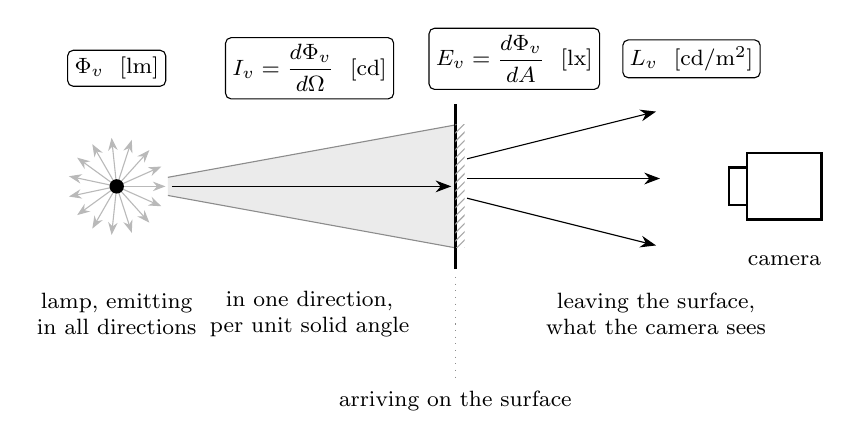
\begin{tikzpicture}[>=Stealth, font=\small, scale=1.0]

% ---- Lamp -------------------------------------------------------------
\foreach \a in {0,24,...,336}{\draw[gray!55,-{Stealth[length=1.6mm]}] (0,0) -- (\a:0.62);}
\fill (0,0) circle (2.6pt);
\node[align=center, font=\footnotesize] at (0,-1.62) {lamp, emitting\\in all directions};
\node[draw, rounded corners=2pt, fill=white, inner sep=2.5pt, font=\footnotesize]
      at (0,1.5) {$\Phi_v$ \ [lm]};

% ---- Solid angle / beam ------------------------------------------------
\fill[black!8] (0.65,0.115) -- (4.3,0.78) -- (4.3,-0.78) -- (0.65,-0.115) -- cycle;
\draw[black!45] (0.65,0.115) -- (4.3,0.78);
\draw[black!45] (0.65,-0.115) -- (4.3,-0.78);
\draw[-{Stealth[length=2mm]}] (0.7,0) -- (4.25,0);
\node[draw, rounded corners=2pt, fill=white, inner sep=2.5pt, font=\footnotesize]
      at (2.45,1.5) {$I_v = \dfrac{d\Phi_v}{d\Omega}$ \ [cd]};
\node[align=center, font=\footnotesize] at (2.45,-1.62) {in one direction,\\per unit solid angle};

% ---- Receiving surface -------------------------------------------------
\draw[line width=1.1pt] (4.3,-1.05) -- (4.3,1.05);
\fill[pattern=north east lines, pattern color=black!35] (4.3,-0.78) rectangle (4.42,0.78);
\node[draw, rounded corners=2pt, fill=white, inner sep=2.5pt, font=\footnotesize]
      at (5.05,1.62) {$E_v = \dfrac{d\Phi_v}{dA}$ \ [lx]};
\draw[black!45, dotted] (4.3,-1.15) -- (4.3,-2.42);
\node[align=center, font=\footnotesize] at (4.3,-2.72) {arriving on the surface};

% ---- Reflected toward the camera --------------------------------------
\draw[-{Stealth[length=2mm]}] (4.45,0.35) -- (6.85,0.95);
\draw[-{Stealth[length=2mm]}] (4.45,0.1) -- (6.9,0.1);
\draw[-{Stealth[length=2mm]}] (4.45,-0.15) -- (6.85,-0.75);
\node[draw, rounded corners=2pt, fill=white, inner sep=2.5pt, font=\footnotesize]
      at (7.3,1.62) {$L_v$ \ [cd/m\textsuperscript{2}]};
\node[align=center, font=\footnotesize] at (6.85,-1.62) {leaving the surface,\\what the camera sees};

% ---- Camera -------------------------------------------------------------
\draw[line width=0.8pt] (8.0,-0.42) rectangle (8.95,0.42);
\draw[line width=0.8pt] (7.78,-0.24) rectangle (8.0,0.24);
\node[font=\footnotesize] at (8.48,-0.95) {camera};

\end{tikzpicture}
\caption[The photometric chain from lamp to sensor]{The photometric chain. The same light is counted four ways: as a total ($\Phi_v$), per unit solid angle ($I_v$), per unit area where it lands ($E_v$), and per unit area and solid angle where it leaves a surface ($L_v$). Only $E_v$ and $L_v$ depend on where the lamp is placed; $\Phi_v$ and $I_v$ are properties of the fixture alone.}
\label{fig:photometric-chain}
\end{figure}

\subsection{Luminous flux, the lumen}

Luminous flux $\Phi_v$ is total radiant power weighted by the eye's spectral response. For a source with spectral radiant flux $\Phi_{e,\lambda}$,

\begin{equation}
\Phi_v = K_m \int_{0}^{\infty} \Phi_{e,\lambda}(\lambda)\, V(\lambda)\, d\lambda ,
\label{eq:lumen}
\end{equation}

where $V(\lambda)$ is the CIE photopic spectral luminous efficiency function \cite{cie_vlambda} and $K_m = 683$~lm/W is the maximum luminous efficacy, the constant that ties the photometric system to the watt through the SI definition of the candela. $V(\lambda)$ peaks at 555~nm and falls to zero outside roughly 380--780~nm, so radiant power in the infrared or the ultraviolet contributes nothing to $\Phi_v$ no matter how much of it there is.

The ratio of the two is the \emph{luminous efficacy of the radiation},

\begin{equation}
K = \frac{\Phi_v}{\Phi_e} \quad \mathrm{[lm/W]} ,
\label{eq:efficacy}
\end{equation}

a property of the source's spectrum. Section \ref{sec:sun-lux} evaluates it for sunlight.

\subsection{Luminous intensity, the candela}

A fixture that concentrates its output into a narrow beam is brighter in that direction than one that spreads the same flux over a hemisphere. Luminous intensity is flux per unit solid angle,

\begin{equation}
I_v = \frac{d\Phi_v}{d\Omega} \quad \mathrm{[lm/sr = cd]} .
\label{eq:candela}
\end{equation}

This is why lumens alone cannot specify this experiment: two fixtures with identical lumen ratings deliver very different light to the tether if their beam angles differ.

\subsection{Illuminance, the lux}

Illuminance is the luminous flux arriving per unit area of a surface,

\begin{equation}
E_v = \frac{d\Phi_v}{dA} \quad \mathrm{[lm/m^2 = lx]} .
\label{eq:lux}
\end{equation}

For a source small enough to be treated as a point, at distance $d$, illuminating a surface whose normal makes an angle $\theta$ with the direction to the source, Equations \ref{eq:candela} and \ref{eq:lux} combine into the inverse-square cosine law,

\begin{equation}
E_v = \frac{I_v \cos\theta}{d^{\,2}} .
\label{eq:inverse-square}
\end{equation}

Equation \ref{eq:inverse-square} is the single most consequential relation in this document: Section \ref{sec:falloff} uses it to show why an uncollimated lamp cannot illuminate the LINKU structure uniformly, and Section \ref{sec:multi-lamp} uses it to rule out lighting the tether end-on.

Illuminance is what a hand-held incident light meter reads when its diffusing dome is placed at the subject position, and it is the quantity this document specifies throughout. In countries using imperial units the same quantity is quoted in foot-candles, where $1~\mathrm{fc} = 1~\mathrm{lm/ft^2} = 10.764~\mathrm{lx}$.

\subsection{Luminance, the nit}

Luminance describes how bright a surface \emph{appears}, which is what a camera actually measures. It is flux per unit projected area per unit solid angle,

\begin{equation}
L_v = \frac{d^2\Phi_v}{dA\,\cos\theta\,d\Omega} \quad \mathrm{[cd/m^2]} .
\label{eq:luminance}
\end{equation}

For the specific case of a Lambertian diffuse reflector, a matte surface that scatters light equally in all directions, of reflectance $\rho$ under illuminance $E_v$, the luminance is

\begin{equation}
L_v = \frac{\rho\, E_v}{\pi} .
\label{eq:lambertian}
\end{equation}

Equation \ref{eq:lambertian} is the bridge between the lighting specification (stated in lux) and the sensor datasheet (stated in cd/m\textsuperscript{2}). Chapter \ref{chap:cameras} uses it in exactly that role. The factor $\pi$, not $2\pi$, follows from integrating the cosine-weighted radiance over the hemisphere.

\subsection{Summary table}

\begin{table}[!ht]
\centering
\small
\caption[Photometric quantities used in this document]{The four photometric quantities, their radiometric counterparts, and their role here.}
\label{tab:quantities}
\begin{tabularx}{\textwidth}{p{0.14\textwidth} p{0.10\textwidth} p{0.17\textwidth} X}
\toprule
\textbf{Quantity} & \textbf{Unit} & \textbf{Radiometric twin} & \textbf{What it answers, and where it is used here} \\
\midrule
Luminous flux $\Phi_v$ & lumen (lm) & radiant flux, W & How much light the lamp makes in total. Quoted in manufacturer catalogues; not a specification for this experiment. \\
Luminous intensity $I_v$ & candela (cd) & radiant intensity, W/sr & How much of it goes in the direction we care about. Implicit in the beam-angle requirement. \\
Illuminance $E_v$ & lux (lx) & irradiance, W/m\textsuperscript{2} & How much light reaches the tether. \textbf{The quantity this document specifies and the experiment measures.} \\
Luminance $L_v$ & cd/m\textsuperscript{2} (nit) & radiance, W/(m\textsuperscript{2}\,sr) & How bright the tether looks to the camera. The quantity image-sensor datasheets are written in. \\
\bottomrule
\end{tabularx}
\end{table}

\section{Exposure arithmetic: stops and EV}
\label{sec:stops}

Lighting and camera work is done in base-2 logarithms of light level. One \emph{stop}, equivalently one unit of exposure value (EV), is a factor of two:

\begin{equation}
\Delta\mathrm{EV} = \log_2\!\left(\frac{E_1}{E_2}\right) .
\label{eq:stops}
\end{equation}

The image a camera forms depends on the product of illuminance and exposure time, the \emph{photometric exposure}

\begin{equation}
H_v = E_v \, t \quad \mathrm{[lx\,s]} ,
\label{eq:exposure}
\end{equation}

so a laboratory source dimmer than the Sun can be compensated by a proportionally longer exposure. That trade has a hard limit in this experiment, because the rotation test of the companion rolling-shutter deliverable caps the usable exposure time; Chapter \ref{chap:cameras} quantifies it.

Expressing a tolerance in stops also makes the uniformity requirement intuitive for a lighting specialist. The IEC non-uniformity definition used in Chapter \ref{chap:sources} compares the brightest and darkest point of the illuminated area; converting that ratio with Equation \ref{eq:stops} gives Table \ref{tab:nu-stops}.

\begin{table}[!ht]
\centering
\small
\caption[IEC non-uniformity classes expressed in photographic stops]{The IEC 60904-9 non-uniformity classes \cite{iec60904_9_2020}, restated as the exposure difference a photographer would read between the brightest and the darkest point of the working area. Computed by \texttt{illumination\_numbers.py}.}
\label{tab:nu-stops}
\begin{tabular}{lccc}
\toprule
\textbf{IEC class} & \textbf{Non-uniformity $NU$} & \textbf{$E_{max}/E_{min}$} & \textbf{Spread in stops} \\
\midrule
A+ & $\leq$1\%  & 1.020 & 0.029~EV \\
A  & $\leq$2\%  & 1.041 & 0.058~EV \\
B  & $\leq$5\%  & 1.105 & 0.144~EV \\
C  & $\leq$10\% & 1.222 & 0.290~EV \\
\bottomrule
\end{tabular}
\end{table}

\section{What a lighting professional actually measures}

Of the four quantities, the one used on set is illuminance in lux, read with an incident light meter at the subject. Catalogue data is published as luminous flux in lumens together with an illuminance-versus-distance table, and colour quality is reported as a correlated colour temperature with a rendering index. The specification in Chapter \ref{chap:spec} is written in exactly these terms, with one acceptance test per line that can be performed with a light meter, a ruler and the project's own cameras.

\chapter{The Reference Sun as a Lighting Fixture}
\label{chap:sun}

This chapter turns the Sun into a set of numbers a lighting specialist can compare a lamp against: how much light it delivers, in lux; how sharp the shadows it casts are, in millimetres of penumbra per metre; and why those two together force a collimated beam rather than simply a bright one.

\section{Nominal solar constants}

Three constants are taken from IAU 2015 Resolution B3, which fixes nominal values for solar quantities so that published work does not drift as measurements are refined \cite{prsa2016iau}:

\begin{table}[!ht]
\centering
\small
\caption[Nominal solar constants used in this document]{Nominal solar constants, IAU 2015 Resolution B3 \cite{prsa2016iau}. The total solar irradiance is quoted there as a solar-cycle-23 mean of $1361 \pm 0.5$~W/m\textsuperscript{2}.}
\label{tab:solar-constants}
\begin{tabularx}{\textwidth}{p{0.235\textwidth} p{0.095\textwidth} p{0.185\textwidth} X}
\toprule
\textbf{Quantity} & \textbf{Symbol} & \textbf{Nominal value} & \textbf{Used in this document for} \\
\midrule
Total solar irradiance   & $\mathcal{S}^{\,\mathrm{N}}_{\odot}$ & 1361 W/m\textsuperscript{2}  & Illuminance of the orbital Sun (Sec. \ref{sec:sun-lux}) \\
Solar radius             & $\mathcal{R}^{\,\mathrm{N}}_{\odot}$ & 695\,700 km                 & Angular diameter, shadow sharpness (Sec. \ref{sec:angular}) \\
Solar effective temperature & $\mathcal{T}^{\,\mathrm{N}}_{\mathrm{eff}\odot}$ & 5772 K       & Target colour temperature (Sec. \ref{sec:colour}) \\
Astronomical unit        & $\mathrm{au}$                        & 149\,597\,870.7 km          & Angular diameter (Sec. \ref{sec:angular}) \\
\bottomrule
\end{tabularx}
\end{table}

\section{From watts per square metre to lux}
\label{sec:sun-lux}

\subsection{The conversion}

Applying the definition of luminous flux, Equation \ref{eq:lumen}, to an irradiance distribution rather than a flux gives the illuminance produced by a spectrum $E_{e,\lambda}$:

\begin{equation}
E_v = K_m \int_{0}^{\infty} E_{e,\lambda}(\lambda)\, V(\lambda)\, d\lambda .
\label{eq:lux-from-spectrum}
\end{equation}

Two primary data sets are required to evaluate it, and both are archived in \texttt{Sources/data/}:

\begin{itemize}
    \item $E_{e,\lambda}(\lambda)$, the ASTM E490-00a standard extraterrestrial (AM0) solar spectral irradiance \cite{astm_e490_data}, tabulated from 119.5~nm upward.
    \item $V(\lambda)$, the CIE photopic spectral luminous efficiency function at 1~nm resolution, CIE 018:2019 Table 1 \cite{cie_vlambda}.
\end{itemize}

Numerically integrating the E490 table by the trapezoidal rule gives a total irradiance of $E_e = 1366.1$~W/m\textsuperscript{2}, and integrating the same table weighted by $V(\lambda)$ gives $E_v = 133\,320$~lx. The ratio is the luminous efficacy of extraterrestrial sunlight, Equation \ref{eq:efficacy}:

\begin{equation}
K_{\mathrm{AM0}} = \frac{133\,320~\mathrm{lx}}{1366.1~\mathrm{W/m^2}} = 97.59~\mathrm{lm/W} .
\label{eq:k-am0}
\end{equation}

The E490 table integrates to 1366.1~W/m\textsuperscript{2} rather than the IAU nominal 1361~W/m\textsuperscript{2}, a difference of 0.37\%, because the two were established at different times against different radiometric scales. Since $K$ is a property of the spectral \emph{shape} and is therefore insensitive to that normalisation, the reported illuminance is obtained by applying Equation \ref{eq:k-am0} to the nominal constant:

\begin{equation}
\boxed{\;E_{v,\odot} = K_{\mathrm{AM0}} \cdot \mathcal{S}^{\,\mathrm{N}}_{\odot}
 = 97.59~\mathrm{lm/W} \times 1361~\mathrm{W/m^2} = 132\,800~\mathrm{lx}\;}
\label{eq:sun-lux}
\end{equation}

at normal incidence, outside the atmosphere. This is the single reference figure against which every lamp considered for the dark room is compared.

\subsection{Why the two unit systems differ so much}

Figure \ref{fig:spectrum} shows the mechanism. The Sun radiates across the whole plotted range, but $V(\lambda)$ is non-zero only in a narrow window, so the integrand of Equation \ref{eq:lux-from-spectrum} is confined to the visible band. Table \ref{tab:bands} gives the fraction of AM0 energy in each band of interest.

\begin{figure}[!ht]
\centering
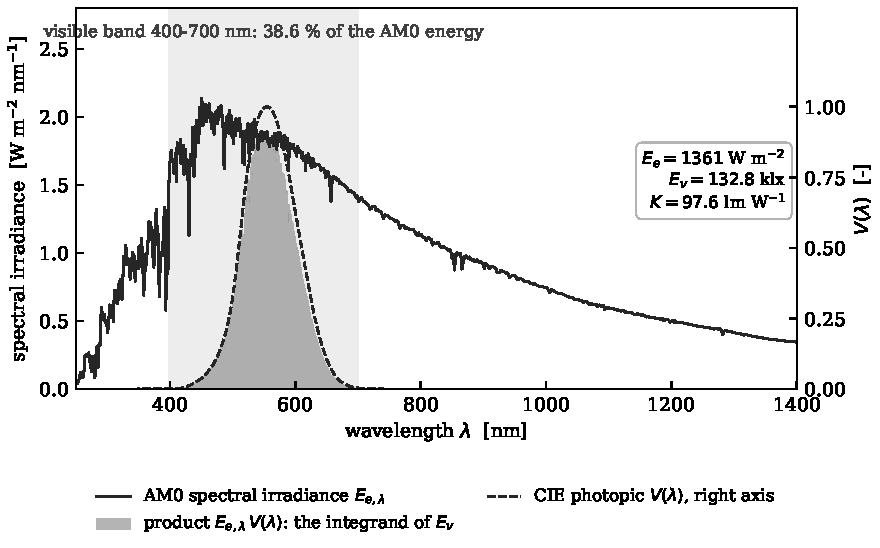
\includegraphics[width=\textwidth]{Images/fig_spectrum_vlambda.pdf}
\caption[AM0 spectral irradiance weighted by the CIE luminous efficiency function]{The AM0 reference spectrum \cite{astm_e490_data}, the CIE photopic luminous efficiency function $V(\lambda)$ \cite{cie_vlambda}, and their product, which is the integrand of Equation \ref{eq:lux-from-spectrum}. The area under the shaded product curve, scaled by $K_m = 683$~lm/W, is the illuminance. Everything the Sun radiates outside the shaded band contributes irradiance but no lux. Generated by \texttt{make\_figures.py} from the archived data files.}
\label{fig:spectrum}
\end{figure}

\begin{table}[!ht]
\centering
\small
\caption[Fraction of AM0 irradiance per wavelength band]{Fraction of the total AM0 irradiance carried by each band, obtained by integrating the E490 table \cite{astm_e490_data}. Computed by \texttt{illumination\_numbers.py}.}
\label{tab:bands}
\begin{tabularx}{\textwidth}{llX}
\toprule
\textbf{Band} & \textbf{Share of $E_e$} & \textbf{Relevance} \\
\midrule
400--700 nm   & 38.6\% & Visible band. Both the Raspberry Pi HQ and Global Shutter cameras carry an infrared filter that reduces sensitivity outside it \cite{raspberrypi_camera_docs}. \\
400--1100 nm  & 66.4\% & Restricted range of the IEC 60904-9 spectral-match classification \cite{iec60904_9_2020}. \\
300--1200 nm  & 77.2\% & Extended range introduced in the 2020 edition, required for class A+ \cite{iec60904_9_2020}. \\
\bottomrule
\end{tabularx}
\end{table}

The practical consequence is that a lamp whose output is heavily weighted toward the infrared can deliver a large irradiance in W/m\textsuperscript{2} while producing few lux and contributing nothing to the image, since the camera's infrared filter discards it. Specifying this experiment in lux rather than W/m\textsuperscript{2} automatically excludes that failure mode.

\section{Colour temperature}
\label{sec:colour}

The Sun's nominal effective temperature is 5772~K \cite{prsa2016iau}, which is why daylight-balanced fixtures are rated near that value. Correlated colour temperature describes the colour of a light source by the temperature of the blackbody radiator it most closely matches; it is not the physical temperature of the lamp. Chapter \ref{chap:sources} shows that every reviewed space laboratory that states a colour temperature uses 5600--6000~K, and Chapter \ref{chap:spec} adopts that range.

\section{Angular diameter and shadow sharpness}
\label{sec:angular}

\subsection{The Sun is not a point source}

From the nominal radius and the astronomical unit, the Sun's angular diameter at 1~au is

\begin{equation}
\alpha_\odot = 2\arctan\!\left(\frac{\mathcal{R}^{\,\mathrm{N}}_{\odot}}{\mathrm{au}}\right)
= 2\arctan\!\left(\frac{695\,700}{149\,597\,870.7}\right) = 0.533^\circ .
\label{eq:angular-diameter}
\end{equation}

This half-degree is what makes orbital shadows look the way they do. A source of finite angular size does not cast a perfectly sharp shadow: behind an occluding edge there is a transition region, the penumbra, which widens with distance from the edge. Figure \ref{fig:penumbra} shows the construction.

\begin{figure}[!ht]
\centering
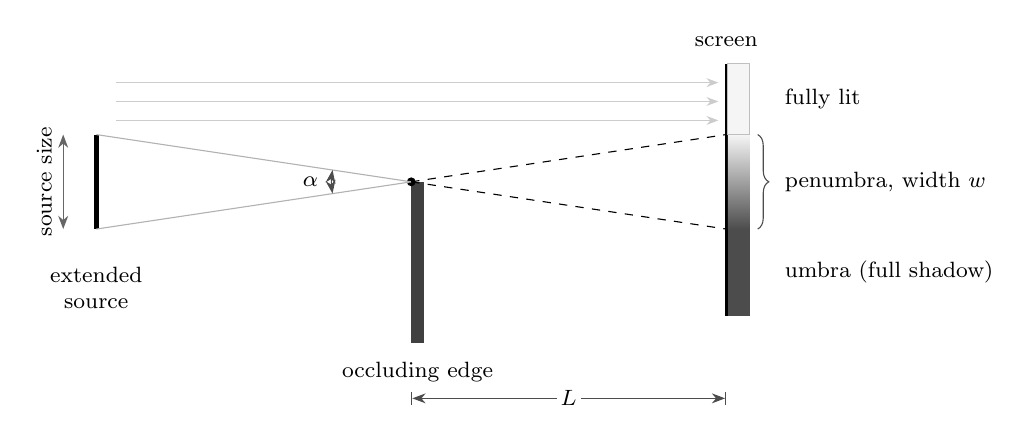
\begin{tikzpicture}[>=Stealth, font=\small, scale=1.0]

% ---- Extended source ----------------------------------------------------
\draw[line width=2pt] (0,-0.6) -- (0,0.6);
\node[align=center, font=\footnotesize] at (0,-1.35) {extended\\source};
\draw[<->, black!60] (-0.42,-0.6) -- (-0.42,0.6);
\node[font=\footnotesize, rotate=90] at (-0.66,0) {source size};

% ---- Occluder -----------------------------------------------------------
\fill[black!75] (4.0,-2.05) rectangle (4.16,0.0);
\node[align=center, font=\footnotesize] at (4.08,-2.42) {occluding edge};
\fill (4.0,0) circle (1.6pt);

% ---- Rays through the tip ----------------------------------------------
\draw[black!30] (0,0.6) -- (4.0,0);
\draw[black!30] (0,-0.6) -- (4.0,0);
\draw[dashed] (4.0,0) -- (8.0,-0.6);
\draw[dashed] (4.0,0) -- (8.0,0.6);
% unobstructed light passing above the edge
\foreach \y in {0.78,1.02,1.26}{\draw[gray!40,-{Stealth[length=1.5mm]}] (0.25,\y) -- (7.9,\y);}

% angle alpha at the tip
\draw[<->, black!70] (3.0,0.15) arc[start angle=171.5, end angle=188.5, radius=1.01];
\node[font=\footnotesize] at (2.72,0) {$\alpha$};

% ---- Screen -------------------------------------------------------------
\draw[line width=1.1pt] (8.0,-1.7) -- (8.0,1.5);
\node[align=center, font=\footnotesize] at (8.0,1.78) {screen};

% shading of the three regions on the screen
\fill[black!70] (8.02,-1.7) rectangle (8.30,-0.6);
\shade[bottom color=black!70, top color=black!4]
      (8.02,-0.6) rectangle (8.30,0.6);
\fill[black!4, draw=black!25] (8.02,0.6) rectangle (8.30,1.5);

\node[font=\footnotesize, anchor=west] at (8.62,-1.15) {umbra (full shadow)};
\node[font=\footnotesize, anchor=west] at (8.62,0.0)   {penumbra, width $w$};
\node[font=\footnotesize, anchor=west] at (8.62,1.05)  {fully lit};

% brace for w
\draw[decorate, decoration={brace, amplitude=4pt}, black!70]
      (8.40,0.6) -- (8.40,-0.6);

% ---- Distance L ---------------------------------------------------------
\draw[|<->|, black!70] (4.0,-2.75) -- (8.0,-2.75);
\node[font=\footnotesize, fill=white, inner sep=1.5pt] at (6.0,-2.75) {$L$};

\end{tikzpicture}
\caption[Penumbra cast by a source of finite angular size]{Penumbra geometry. The two rays that graze the occluding edge come from opposite edges of the source and therefore diverge by the source's angular size $\alpha$; at a distance $L$ behind the edge they are separated by $w = L\tan\alpha$. The angle $\alpha$ is drawn greatly exaggerated for legibility: at the real solar value of $0.533^\circ$ the two dashed rays would be visually indistinguishable. The construction shown is internally consistent, with $\alpha = 17.1^\circ$ as drawn.}
\label{fig:penumbra}
\end{figure}

\subsection{The penumbra relation}

From the construction in Figure \ref{fig:penumbra}, the penumbra width at a distance $L$ behind the occluding edge is

\begin{equation}
w = L \tan\alpha .
\label{eq:penumbra}
\end{equation}

Evaluating Equation \ref{eq:penumbra} at $\alpha_\odot$ gives $w/L = 9.3$~mm per metre for real sunlight. Table \ref{tab:penumbra} lists the same quantity for the beam divergences that appear later in this document. This relation is the basis of the acceptance test in Chapter \ref{chap:spec}, because it converts an angular specification, which needs optical instruments to verify, into a length measurable with a ruler.

\begin{table}[!ht]
\centering
\small
\caption[Penumbra width per metre for several source angular sizes]{Penumbra width per metre of distance behind the occluding edge, from Equation \ref{eq:penumbra}. Computed by \texttt{illumination\_numbers.py}.}
\label{tab:penumbra}
\begin{tabularx}{\textwidth}{p{0.17\textwidth} X c}
\toprule
\textbf{Angular size $\alpha$} & \textbf{Reference} & \textbf{$w/L$ [mm/m]} \\
\midrule
0.53\textdegree & the real Sun at 1 au, Eq. \ref{eq:angular-diameter} & 9.3 \\
1.00\textdegree & -- & 17.5 \\
1.90\textdegree & collimation angle of the ESA Large Space Simulator beam \cite{esa_lss} & 33.2 \\
2.00\textdegree & limit adopted for LINKU, Chapter \ref{chap:spec} & 34.9 \\
5.00\textdegree & a typical uncollimated spotlight & 87.5 \\
\bottomrule
\end{tabularx}
\end{table}

\section{Why collimation, not merely distance}
\label{sec:falloff}

\subsection{The problem}

The LINKU structure occupies a volume, not a plane. A lamp small enough to be treated as a point illuminates the near and far faces of that volume unequally, by the inverse-square law of Equation \ref{eq:inverse-square}. Figure \ref{fig:falloff} defines the geometry.

\begin{figure}[!ht]
\centering
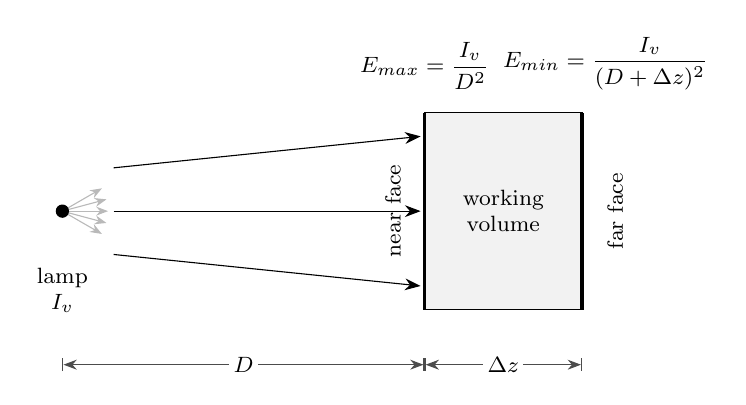
\begin{tikzpicture}[>=Stealth, font=\small, scale=1.0]

% lamp
\foreach \a in {-30,-15,...,30}{\draw[gray!55,-{Stealth[length=1.5mm]}] (0,0) -- (\a:0.58);}
\fill (0,0) circle (2.4pt);
\node[font=\footnotesize, align=center] at (0,-1.0) {lamp\\$I_v$};

% working volume
\draw[fill=black!5] (4.6,-1.25) rectangle (6.6,1.25);
\node[align=center, font=\footnotesize] at (5.6,0.0) {working\\volume};

% near and far faces
\draw[line width=1.3pt] (4.6,-1.25) -- (4.6,1.25);
\draw[line width=1.3pt] (6.6,-1.25) -- (6.6,1.25);
\node[font=\footnotesize, rotate=90, anchor=south] at (4.42,0) {near face};
\node[font=\footnotesize, rotate=90, anchor=north] at (6.80,0) {far face};

% rays
\draw[-{Stealth[length=2mm]}] (0.65,0.55) -- (4.55,0.95);
\draw[-{Stealth[length=2mm]}] (0.65,0) -- (4.55,0);
\draw[-{Stealth[length=2mm]}] (0.65,-0.55) -- (4.55,-0.95);

% distances
\draw[|<->|, black!70] (0,-1.95) -- (4.6,-1.95);
\node[font=\footnotesize, fill=white, inner sep=1.5pt] at (2.3,-1.95) {$D$};
\draw[|<->|, black!70] (4.6,-1.95) -- (6.6,-1.95);
\node[font=\footnotesize, fill=white, inner sep=1.5pt] at (5.6,-1.95) {$\Delta z$};

% illuminance labels
\node[font=\footnotesize, anchor=south] at (4.6,1.42) {$E_{max} = \dfrac{I_v}{D^{2}}$};
\node[font=\footnotesize, anchor=south] at (6.9,1.42) {$E_{min} = \dfrac{I_v}{(D+\Delta z)^{2}}$};

\end{tikzpicture}
\caption[Inverse-square falloff across the depth of the working volume]{An uncollimated point source at throw $D$ illuminates the near face of a working volume of depth $\Delta z$ more strongly than the far face, in the ratio $\left(D/(D+\Delta z)\right)^{2}$. A collimated beam does not spread with distance and so does not produce this gradient.}
\label{fig:falloff}
\end{figure}

\subsection{Quantifying it against the IEC criterion}

IEC 60904-9 defines spatial non-uniformity over the designated test area as \cite{iec60904_9_2020}

\begin{equation}
NU = \frac{E_{max} - E_{min}}{E_{max} + E_{min}} \times 100\,\% .
\label{eq:nu}
\end{equation}

Substituting the two illuminances of Figure \ref{fig:falloff} and writing $r = E_{min}/E_{max} = \left(D/(D+\Delta z)\right)^{2}$,

\begin{equation}
NU = \frac{1-r}{1+r} .
\label{eq:nu-r}
\end{equation}

Inverting Equation \ref{eq:nu-r} for the throw required to meet a given non-uniformity, with $r = (1-NU)/(1+NU)$, gives

\begin{equation}
D_{\min} = \Delta z \cdot \frac{\sqrt{r}}{1-\sqrt{r}} .
\label{eq:dmin}
\end{equation}

Table \ref{tab:falloff} evaluates both relations. The result is restrictive: holding class B uniformity with an uncollimated lamp requires a throw of about twenty times the depth of the object, which for a structure 0.5~m deep means roughly 10~m of clear space, and for a 1~m depth roughly 20~m. Few dark rooms offer that, and at the distances that are available the gradient is already outside class C.

\begin{table}[!ht]
\centering
\small
\caption[Throw required for a given uniformity, and uniformity obtained at a given throw]{Left: minimum throw from Equation \ref{eq:dmin}, as a multiple of the working-volume depth. Right: non-uniformity from Equation \ref{eq:nu-r} at throws a dark room might realistically allow. Computed by \texttt{illumination\_numbers.py}.}
\label{tab:falloff}
\setlength{\tabcolsep}{4pt}
\begin{tabular}{llc@{\hskip 0.7cm}llc}
\toprule
\multicolumn{3}{c}{\textbf{Throw required}} & \multicolumn{3}{c}{\textbf{Uniformity obtained}} \\
\cmidrule(r){1-3}\cmidrule(l){4-6}
\textbf{Target} & \textbf{IEC class} & \textbf{$D_{\min}$} & \textbf{$D$} & \textbf{$\Delta z$} & \textbf{$NU$} \\
\midrule
$NU \leq 2\%$  & A & $49.5\,\Delta z$ & 3 m  & 0.5 m & 15.3\% \\
$NU \leq 5\%$  & B & $19.5\,\Delta z$ & 5 m  & 0.5 m & 9.5\% \\
$NU \leq 10\%$ & C & $9.5\,\Delta z$  & 10 m & 0.5 m & 4.9\% \\
               &   &                  & 5 m  & 1.0 m & 18.0\% \\
               &   &                  & 10 m & 1.0 m & 9.5\% \\
\bottomrule
\end{tabular}
\end{table}

\subsection{The conclusion that follows}

An ideally collimated beam consists of parallel rays and therefore does not spread with distance, so Equation \ref{eq:inverse-square} does not apply to it and the gradient of Table \ref{tab:falloff} disappears. This is why the requirement in Chapter \ref{chap:spec} is for a collimated or near-parallel beam rather than simply a bright lamp placed far away, and it is consistent with what the reviewed facilities did: the ESA Large Space Simulator specifies a collimation angle for its sun beam \cite{esa_lss}, and the SnT Zero-G Lab selected a collimator specifically to mimic sunlight without atmosphere \cite{pauly2022spacelab}.

\todo[inline]{Pending: measure the working-volume depth $\Delta z$ of the LINKU structure and the maximum lamp throw $D$ available in the dark room, then evaluate Equations \ref{eq:nu-r} and \ref{eq:dmin} for those specific values before the room is booked.}

\chapter{How Solar Simulation Is Graded, and What Comparable Laboratories Built}
\label{chap:sources}

Two bodies of practice bear on this experiment. The photovoltaic industry has a formal standard for grading solar simulators, which supplies rigorous definitions and numeric thresholds. Spacecraft vision-based navigation laboratories have no such standard but have repeatedly solved the same problem this experiment faces, and their published descriptions show what is actually built. This chapter takes the definitions and thresholds from the first and the engineering practice from the second, and is explicit about which claims could be traced to a facility's own operators.

\section{IEC 60904-9: the photovoltaic classification}

\subsection{What the standard grades}

IEC 60904-9 classifies a solar simulator on exactly three measurable properties: how closely its output spectrum matches a reference solar spectrum, how uniform its irradiance is across the test plane, and how stable that irradiance is in time \cite{iec60904_9_2020}. A simulator is rated with three letters in that order, so that a ``CBA'' simulator has a class C spectral match, class B spatial non-uniformity and class A temporal instability.

Only the free official preview of the standard, covering clauses 1 to 5.2 and including all three tables reproduced below, was read for this document. The measurement procedures that follow clause 5.2 remain behind the paywall.

\begin{table}[!ht]
\centering
\small
\caption[IEC 60904-9:2020 solar simulator classifications]{Solar simulator classifications, Table 3 of IEC 60904-9:2020 Edition 3.0 \cite{iec60904_9_2020}. STI and LTI are short- and long-term temporal instability. Class A+ was introduced in the 2020 edition and is only defined when spectral match is evaluated in the extended wavelength range of Table \ref{tab:iec-bands-ext}.}
\label{tab:iec-classes}
\begin{tabular}{lcccc}
\toprule
\textbf{Class} & \textbf{Spectral match, all intervals} & \textbf{Spatial non-uniformity} & \textbf{STI} & \textbf{LTI} \\
\midrule
A+  & 0.875--1.125$\times$ reference & $\leq$1\%  & $\leq$0.25\% & $\leq$1\% \\
A   & 0.75--1.25$\times$ reference   & $\leq$2\%  & $\leq$0.5\%  & $\leq$2\% \\
B   & 0.6--1.4$\times$ reference     & $\leq$5\%  & $\leq$2\%    & $\leq$5\% \\
C   & 0.4--2.0$\times$ reference     & $\leq$10\% & $\leq$10\%   & $\leq$10\% \\
\bottomrule
\end{tabular}
\end{table}

Two parts of the standard are used directly in this document. The non-uniformity definition, Equation \ref{eq:nu}, is adopted as the uniformity criterion in Chapter \ref{chap:spec}, and the class B thresholds are adopted as the LINKU targets. The standard also states explicitly that a classification is valid only for the conditions under which it was measured, and lists ``reflections from the surroundings such as properties of dark room walls'' among the factors that change it \cite{iec60904_9_2020}, which is a direct warning for a dark-room experiment.

\subsection{The spectral-match intervals}

For the spectral match, the reference AM1.5G spectrum is divided into six wavelength intervals, and the simulator's share of total irradiance in each interval must fall within the ratios of Table \ref{tab:iec-classes}. The 2020 edition defines two interval sets: the restricted set retained for backward compatibility (Table \ref{tab:iec-bands-restricted}) and the extended set required for class A+ (Table \ref{tab:iec-bands-ext}).

\begin{table}[!ht]
\centering
\small
\begin{minipage}[t]{0.48\textwidth}
\centering
\caption[AM1.5G intervals, restricted range]{Table 1 of \cite{iec60904_9_2020}: restricted range, 400--1100 nm.}
\label{tab:iec-bands-restricted}
\begin{tabular}{ccc}
\toprule
\textbf{\#} & \textbf{Range [nm]} & \textbf{Share [\%]} \\
\midrule
1 & 400--500   & 18.4 \\
2 & 500--600   & 19.9 \\
3 & 600--700   & 18.4 \\
4 & 700--800   & 14.9 \\
5 & 800--900   & 12.5 \\
6 & 900--1100  & 15.9 \\
\bottomrule
\end{tabular}
\end{minipage}
\hfill
\begin{minipage}[t]{0.48\textwidth}
\centering
\caption[AM1.5G intervals, extended range]{Table 2 of \cite{iec60904_9_2020}: extended range, 300--1200 nm, required for A+.}
\label{tab:iec-bands-ext}
\begin{tabular}{ccc}
\toprule
\textbf{\#} & \textbf{Range [nm]} & \textbf{Share [\%]} \\
\midrule
1 & 300--470   & 16.61 \\
2 & 470--561   & 16.74 \\
3 & 561--657   & 16.67 \\
4 & 657--772   & 16.63 \\
5 & 772--919   & 16.66 \\
6 & 919--1200  & 16.69 \\
\bottomrule
\end{tabular}
\end{minipage}
\end{table}

\subsection{Why only part of the standard applies here}

The spectral-match criterion is designed for photovoltaic testing, where the quantity of interest is the electrical energy a cell harvests across its full spectral response, extending well into the infrared. LINKU's instrument is a camera with an infrared filter \cite{raspberrypi_camera_docs}, so three of the six intervals in Table \ref{tab:iec-bands-restricted} lie largely outside the band it records. The uniformity and stability criteria, by contrast, transfer directly: a gradient or a fluctuation degrades an image exactly as it degrades a cell measurement. Chapter \ref{chap:spec} therefore adopts the IEC definitions and thresholds for uniformity and stability, and replaces the spectral-match criterion with a colour-temperature and colour-rendering requirement drawn from the laboratory practice reviewed below.

\section{Light-source technologies}

Three technologies dominate solar simulator design. Table \ref{tab:tech} summarises the trade, grounded in the comparative review inside \cite{rezende2024lowcost} and the LED testbed of \cite{schulthess2026classaaa}.

\begin{table}[!ht]
\centering
\small
\caption[Solar simulator light-source technologies]{Light-source technologies for solar simulation.}
\label{tab:tech}
\begin{tabularx}{\textwidth}{p{0.16\textwidth} X X}
\toprule
\textbf{Technology} & \textbf{Spectral quality} & \textbf{Cost and practical notes} \\
\midrule
Xenon arc & Best broadband match to the solar spectrum, including the ultraviolet; the industry reference for class AAA systems. & Most expensive per watt; needs housing, filtering and lamp replacement. Normally justified only for a dedicated photovoltaic testing laboratory. \\
Metal halide / HMI & Matches natural sunlight satisfactorily per prior work, at far lower cost per watt than xenon arc. & A published large-area design used seven 1500~W stadium fixtures for a total build cost below \$10\,000 \cite{rezende2024lowcost}. This is also the family used as the sun simulator at DLR EPOS and at Stanford TRON (Table \ref{tab:vision-labs}). \\
LED array & Spectrum is tunable by combining emitters of different peak wavelengths rather than fixed by one emitter. Reaches class AAA when actively controlled and calibrated \cite{schulthess2026classaaa}. & Cheapest, most compact and most controllable; the technology recommended by every LED-based precedent reviewed. Reaching class AAA requires closed-loop spectral sensing. \\
\bottomrule
\end{tabularx}
\end{table}

Two LED builds bracket the achievable range. Rezende et al. built a 2U CubeSat electrical-power-system test bench from 10 white LEDs of about 10~W each, driven at 36~V and sized to deliver 1000~W/m\textsuperscript{2} at the device under test, inside a 440$\times$340$\times$340~mm wooden box; all ten emitters are the same white type, current-controlled for intensity only, with no spectral tuning \cite{rezende2024lowcost}. Schulthess et al. built a verified class AAA testbed from 2964 LEDs of 8 distinct types, including infrared peaks at 740, 850 and 940~nm, closed-loop against an 18-channel spectrometer, reaching a spectral match below 1.3\% and non-uniformity below 1.28\% over a 16.5$\times$16.5~cm area \cite{schulthess2026classaaa}. The gap between these two builds is the cost of spectral fidelity, and it is a cost this experiment does not need to pay, because what the LINKU cameras require is directional geometry and stable level, not a photovoltaic-grade spectrum.

\section{Spacecraft vision laboratories}
\label{sec:vision-labs}

Laboratories that photograph spacecraft mock-ups under simulated sunlight face the same problem as this experiment. The starting point for this section is the facility survey of Pauly et al. \cite{pauly2022spacelab}; each facility was then checked against a document written by its own operators wherever an open copy could be obtained. Table \ref{tab:vision-labs} reports the result and labels the source level of every row.

\begin{table}[!ht]
\centering
\small
\caption[Sun simulation in spacecraft vision laboratories]{Sun simulation in spacecraft vision-based navigation laboratories. ``Primary'' means the values were read in a document written by the facility's own operators; ``secondary'' means they rest only on the survey \cite{pauly2022spacelab}.}
\label{tab:vision-labs}
\begin{tabularx}{\textwidth}{p{0.15\textwidth} X p{0.17\textwidth}}
\toprule
\textbf{Facility} & \textbf{Sun source and reported characteristics} & \textbf{Source level} \\
\midrule
ESA Large Space Simulator, ESTEC & Collimated sun beam of 6~m diameter, 70--2600~W/m\textsuperscript{2}, collimation angle 1.9\textdegree, in-plane uniformity $\pm$4\%, in-volume $\pm$6\%, stability $\pm$0.5\% at one solar constant. & Primary \cite{esa_lss} \\
DLR EPOS 2.0, Germany & ARRI Max 12/18 spotlight with a 12~kW Osram HMI lamp, luminous flux 1.15 million lumens, daylight colour temperature 6000~K, colour rendering index 90. Spectrally verified against sunlight with a spectral irradiance meter at 7~m. Operating distance 7--10~m, chosen according to the sensor's spectral sensitivity. Black molton curtain, carpet and robot wrapping. & Primary \cite{benninghoff2017epos,dlr2025eposportfolio} \\
Stanford TRON, USA & Metal halide arc lamp for direct sunlight, plus 10 LED light boxes for Earth albedo. All ambient sources covered with black commando curtains. The sun lamp casts a flare across the image when the camera points near it. & Primary \cite{park2021tron} \\
FIT ORION, USA & Litepanels Hilio D12 LED panel, 350~W, 5600~K, used to create orbital lighting effects. The beam angle of 10--60\textdegree, continuous dimming and low-reflectivity black paint on walls, floor and ceiling are reported only in the survey. & Primary for fixture, power and colour temperature \cite{mahendrakar2023orion}; secondary for the rest \cite{pauly2022spacelab} \\
SnT Zero-G Lab, Luxembourg & Godox SL-60 LED, 5600~K, tested bare, with reflector and with collimator; the collimated configuration was chosen to mimic the Sun without atmosphere. Black velvet scored best among the background materials tested, using the Raspberry Pi HQ camera. & Primary \cite{pauly2022spacelab} \\
DFKI INVERITAS, Germany & Six motorised 575~W gas-discharge spotlights, 6000~K, maximum 14\,500~lx at 10~m with a 12\textdegree{} field; light-absorbing paint on walls and components. & Secondary \cite{pauly2022spacelab}; the original \cite{paul2015inveritas} is paywalled and the open copy refused automated download \\
ESA GRALS, ESTEC & Dimmable collimated lamp with spectral response close to 6000~K and uniformity $\pm$5\%. & Secondary \cite{pauly2022spacelab}; the cited original \cite{cassinis2022grals} refused automated download, and its open conference version does not describe the lamp \\
\bottomrule
\end{tabularx}
\end{table}

\subsection{Corrections found during verification}

Checking against the originals changed two entries, which is the reason the source-level column exists:

\begin{itemize}
    \item \textbf{EPOS.} The survey describes an ``ARRI Max 18/12 \dots mounted on a 2-DOF yoke'' \cite{pauly2022spacelab}. Neither operator document read here uses that designation or mentions a yoke; both name the fixture ARRI Max 12/18 and give the 12~kW lamp, 6000~K and CRI 90 figures reported in Table \ref{tab:vision-labs} \cite{benninghoff2017epos,dlr2025eposportfolio}.
    \item \textbf{TRON.} A web summary consulted during the search described the sun lamp as a xenon short-arc lamp. The operators' own paper states a metal halide arc lamp \cite{park2021tron}, and that is what Table \ref{tab:vision-labs} reports.
\end{itemize}

The GRALS description in the survey ends with the phrase ``shadow-free backlight illumination'', wording that does not describe a sun simulator. It is reported for completeness and given no weight in this document.

\subsection{What the facilities agree on}

None of these laboratories attempts a photovoltaic-grade spectral match. They converge instead on four properties, and these four are what Chapter \ref{chap:spec} turns into requirements:

\begin{enumerate}
    \item A single hard, directional source representing the Sun.
    \item A daylight colour temperature between 5600 and 6000~K.
    \item A black, light-absorbing environment with no ambient light and the fixture out of the camera's field.
    \item A collimated or narrow beam, wherever the beam geometry is specified at all.
\end{enumerate}

\subsection{A scale reference for intensity}
\label{sec:epos-scale}

The DLR portfolio document includes a figure plotting the absolute spectral irradiance of the 12~kW HMI spotlight at 7~m and at 10~m against sunlight in Earth orbit, over roughly 400--1050~nm \cite{dlr2025eposportfolio}. Read from that figure, the 7~m curve lies above the solar curve across most of the visible band and the 10~m curve lies below it. A fixture of that class therefore brackets one solar constant somewhere between 7 and 10~m, which is the only published order-of-magnitude anchor found for what full-Sun intensity costs in hardware. Chapter \ref{chap:cameras} shows that the LINKU experiment does not need anything close to that level.

\chapter{Camera-Side Requirements}
\label{chap:cameras}

Chapters \ref{chap:sun} and \ref{chap:sources} describe the light. This chapter describes what the instrument needs from it. The chain is short: the optics fix how much of the scene each pixel sees; the rotation test fixes how long the shutter may stay open; the sensor datasheet fixes how much light must arrive in that time; and the supply waveform fixes whether that light may flicker.

\section{The cameras and the optics}

\subsection{Which lens is actually fitted}

The IMX477 stereo pair in use today carries the \textbf{Arducam C1508ZM04, 8~mm focal length, F1.6 to F16 adjustable, C-mount}, not the 6~mm wide-angle lens that ships with the Raspberry Pi HQ camera. This is the configuration recorded in the LINKU D5 Camera System Report \cite{linku_d5_camera_report}, which states that an 8~mm focal length was selected for the experimental validation campaign and that each sensor was equipped with that lens, and it is the focal length used in the rolling-shutter deliverable's own IFOV estimate. Every requirement in this chapter is therefore anchored on the 8~mm configuration.

The project owns three interchangeable C/CS-mount lenses, listed in Table \ref{tab:lenses}, and the Hawk-eye can take none of them: it is a sealed autofocus module with an integrated 5.1~mm F1.8 optic. Because the choice of lens turns out to be the largest single term in the light budget, all six combinations are carried through this chapter rather than only the fitted one, so that the consequence of a future swap can be read off directly.

\begin{table}[!ht]
\centering
\small
\caption[Lenses available to the project]{The three interchangeable lenses the project owns, plus the Hawk-eye's fixed optic. Adjustable lenses are evaluated wide open, which is the best case for light; stopping down for depth of field costs light as $N^{2}$ (Equation \ref{eq:ltsat-n}).}
\label{tab:lenses}
\footnotesize
\setlength{\tabcolsep}{4pt}
\begin{tabularx}{\textwidth}{>{\raggedright\arraybackslash}p{0.165\textwidth} p{0.105\textwidth} p{0.065\textwidth} p{0.075\textwidth} X}
\toprule
\textbf{Lens} & \textbf{Aperture} & \textbf{Mount} & \textbf{M.O.D.} & \textbf{Status} \\
\midrule
Arducam C1508ZM04, 8 mm & F1.6--F16 & C & 0.15 m & \textbf{Fitted to the IMX477 pair today} \\
Raspberry Pi 6 mm wide & F1.2 fixed & CS & 0.2 m & Shipped with the HQ camera; retained \\
Telephoto 16 mm & F1.4--F16 & C & 0.2 m & Quoted with the IMX296; previously excluded \\
Hawk-eye integrated, 5.1 mm & F1.8 fixed & none & 0.08 m & Not interchangeable \\
\bottomrule
\end{tabularx}
\end{table}

Every minimum object distance in Table \ref{tab:lenses} is far below the 3.5~m dark-room working distance, so focusing is not a constraint for any configuration.

\begin{table}[!ht]
\centering
\small
\caption[Candidate cameras and their fixed parameters]{The three candidate cameras. Active sensor width is derived as pixel pitch times horizontal resolution, so that all geometry in this chapter rests on the same two published numbers per sensor.}
\label{tab:cameras}
\begin{tabularx}{\textwidth}{p{0.155\textwidth} p{0.13\textwidth} p{0.115\textwidth} p{0.125\textwidth} p{0.085\textwidth} X}
\toprule
\textbf{Camera} & \textbf{Sensor} & \textbf{Pixel pitch} & \textbf{Resolution} & \textbf{Shutter} & \textbf{Lenses evaluated} \\
\midrule
Raspberry Pi HQ   & Sony IMX477 & 1.55 \textmu m & 4056$\times$3040 & rolling & 8 mm (fitted), 6 mm \\
Raspberry Pi GS   & Sony IMX296 & 3.45 \textmu m & 1456$\times$1088 & global  & 16 mm, 8 mm, 6 mm \\
Arducam 64MP Hawk-eye & not identified by the manufacturer & 0.80 \textmu m & 9152$\times$6944 & rolling & 5.1 mm, fixed \\
\bottomrule
\end{tabularx}
\end{table}

Sources: pitch, resolution and shutter type for the two Raspberry Pi cameras from the official camera documentation \cite{raspberrypi_camera_docs}, and for the Hawk-eye from the Arducam wiki \cite{arducam_hawkeye_wiki}, which states the optical format as type 1/1.7'' but does not name the sensor die. Lens data: the 8~mm from the Arducam C1508ZM04 specification \cite{arducam_c1508zm04} and the D5 Camera System Report \cite{linku_d5_camera_report}; the 6~mm from the Raspberry Pi recommended-lens table \cite{raspberrypi_camera_docs}; the 16~mm and the Hawk-eye's integrated optic from the project's own optical comparator.

The IMX296 is a candidate sensor, not installed hardware, so its three rows below are projections rather than measurements of an existing rig.

\subsection{A note on the project's optical comparator}

\texttt{camera\_dof\_visualizer.py} labels the Hawk-eye entry as sensor ``OV64A40'' with a pixel pitch of 1.4~\textmu m marked as estimated. The OV64A40 is a different Arducam product, the 64MP OwlSight, of optical format 1/1.32''. The Hawk-eye's documented pitch is 0.80~\textmu m \cite{arducam_hawkeye_wiki}, which is also what pitch equals when derived from that file's own sensor width and resolution, so the comparator's computed outputs are unaffected; only the label and the comment are wrong. A second discrepancy is recorded in Appendix \ref{app:findings}.

\section{Angular and spatial sampling}

Four quantities follow from the pitch $p$, the focal length $f$, the active width $W = p \cdot N_h$ and the working distance $D$. The instantaneous field of view of one pixel, in the small-angle limit that holds for every configuration here, is

\begin{equation}
\mathrm{IFOV} = \frac{p}{f} ,
\label{eq:ifov}
\end{equation}

the horizontal field of view of the whole sensor is

\begin{equation}
\mathrm{FOV}_H = 2\arctan\!\left(\frac{W}{2f}\right) ,
\label{eq:fov}
\end{equation}

the ground sample distance, the size of the scene patch imaged onto one pixel at distance $D$, is

\begin{equation}
\mathrm{GSD} = \frac{p\,D}{f} = D \cdot \mathrm{IFOV} ,
\label{eq:gsd}
\end{equation}

and the number of pixels across a tether of diameter $d$ is

\begin{equation}
n_{px} = \frac{d}{\mathrm{GSD}} .
\label{eq:npx}
\end{equation}

Table \ref{tab:sampling} evaluates these at the stereo working distance of 3.5~m used in the enclosure replica, for the 1~mm tether diameter that is the default in the project's optical comparator.

\begin{table}[!ht]
\centering
\small
\caption[Sampling geometry of the six configurations]{Sampling geometry at a working distance of $D = 3.5$~m, tether diameter $d = 1$~mm. Computed by \texttt{illumination\_numbers.py} from Equations \ref{eq:ifov} to \ref{eq:npx}.}
\label{tab:sampling}
\begin{tabular}{lccccc}
\toprule
\textbf{Configuration} & \textbf{$W$ [mm]} & \textbf{IFOV [\textdegree]} & \textbf{$\mathrm{FOV}_H$ [\textdegree]} & \textbf{GSD [mm]} & \textbf{$n_{px}$} \\
\midrule
\textbf{IMX477 + 8 mm F1.6 (fitted)} & \textbf{6.287} & \textbf{0.0111} & \textbf{42.9} & \textbf{0.678} & \textbf{1.47} \\
IMX477 + 6 mm F1.2            & 6.287 & 0.0148 & 55.3 & 0.904 & 1.11 \\
IMX296 + 16 mm F1.4           & 5.023 & 0.0124 & 17.8 & 0.755 & 1.33 \\
IMX296 + 8 mm F1.6            & 5.023 & 0.0247 & 34.9 & 1.509 & 0.66 \\
IMX296 + 6 mm F1.2            & 5.023 & 0.0329 & 45.4 & 2.013 & 0.50 \\
Hawk-eye + 5.1 mm F1.8        & 7.322 & 0.0090 & 71.3 & 0.549 & 1.82 \\
\bottomrule
\end{tabular}
\end{table}

Two independent checks validate the geometry. For the 6~mm lens, the derived 55.3\textdegree{} and 45.4\textdegree{} reproduce the manufacturer's published 55\textdegree{} and 45\textdegree{} for that lens on those two cameras \cite{raspberrypi_camera_docs}. For the fitted 8~mm lens, the derived 42.9\textdegree{} agrees with the 44\textdegree{} horizontal that Arducam publishes for the C1508ZM04 on a 1/2.3'' IMX477 \cite{arducam_c1508zm04}, the small residual being the difference between the nominal 1/2.3'' format width and the 6.287~mm active width derived here.

The last column confirms the regime the project already works in: at 3.5~m the tether spans 1.47 pixels in the fitted configuration, and less than that in four of the other five. A target that thin leaves no margin for a blurred or banded image, which is why the two constraints that follow are stated as hard limits rather than preferences.

\paragraph{Why published field-of-view figures must be checked against the sensor.} A lens specification states a field of view for the optical format the lens was designed to cover, which is usually larger than the sensor actually behind it, and the figure is sometimes a diagonal rather than a horizontal. Both traps appear in the specifications of the lenses used here.

\begin{table}[!ht]
\centering
\small
\caption[Published versus derived field of view]{Published field-of-view figures against the value derived from Equation \ref{eq:fov} with the IMX477's 6.287~mm active width. The derived column is what this document uses, because it is the only one tied to the sensor actually in the camera.}
\label{tab:fov-check}
\begin{tabularx}{\textwidth}{p{0.12\textwidth} p{0.16\textwidth} p{0.14\textwidth} p{0.11\textwidth} X}
\toprule
\textbf{Lens} & \textbf{Published} & \textbf{Source} & \textbf{Derived} & \textbf{Reading} \\
\midrule
8 mm & 58.4\textdegree(H) $\times$ 44.6\textdegree(V) & Arducam, for 2/3'' \cite{arducam_c1508zm04} & 57.6\textdegree{} on 2/3'' & Correct, but for a format larger than this sensor \\
8 mm & 44\textdegree(H) on 1/2.3'' & Arducam \cite{arducam_c1508zm04} & \textbf{42.9\textdegree} & Agrees; this is the figure to use \\
6 mm & 55\textdegree $\times$ 45\textdegree{} (71\textdegree{} diag.) & Raspberry Pi \cite{raspberrypi_camera_docs} & \textbf{55.3\textdegree} & Agrees \\
6 mm & 65\textdegree(H) & Arducam, HQ bundle B0240 & 66.4\textdegree{} \emph{diagonal} & Disagrees with the horizontal; matches the diagonal \\
\bottomrule
\end{tabularx}
\end{table}

The 6~mm row is the one worth dwelling on, because the two vendors disagree by 10\textdegree{} for the same focal length on the same sensor. The Arducam page that quotes 65\textdegree(H) also states the sensor image area as 6.287$\times$4.712~mm on the same page, and those two statements are not compatible: a rectilinear 6~mm lens over a 6.287~mm width subtends 55.3\textdegree, and reaching a true 65\textdegree{} horizontal would require a sensor 7.64~mm wide. What 7.64~mm is close to is the IMX477's 7.86~mm \emph{diagonal}, which subtends 66.4\textdegree. The most likely explanation is a diagonal figure labelled as horizontal. A real alternative exists, since a wide-angle lens with barrel distortion can capture a field wider than the paraxial formula predicts, but that would not explain Raspberry Pi publishing 55\textdegree{} for the same focal length on the same camera, nor the fact that Arducam's own 8~mm figure for this sensor does follow the geometric convention.

This document uses the derived values throughout. The choice is low-risk: \textbf{no other quantity in this chapter depends on the field of view.} The instantaneous field of view, ground sample distance, tether sampling, exposure ceiling and illuminance requirement all follow from pixel pitch and focal length alone, through Equations \ref{eq:ifov}, \ref{eq:gsd}, \ref{eq:tmax} and \ref{eq:emin}. Field of view matters only for framing, so if the real coverage of the 6~mm lens becomes relevant it should be measured on site rather than taken from either vendor page.

Appendix \ref{app:findings} records where these published figures have propagated into the project's own documentation and code.

\section{The exposure ceiling imposed by rotation}

\subsection{Relation}

During the rotation test the camera turns at angular rate $\omega$ while the shutter is open, so the image of a stationary object sweeps across the sensor. In angular terms the image moves by $\omega t$ during an exposure of duration $t$, and dividing by the angle one pixel subtends gives the blur in pixels,

\begin{equation}
b = \frac{\omega\,t}{\mathrm{IFOV}} .
\label{eq:blur}
\end{equation}

Requiring the blur to stay within a budget of $b_{\max}$ pixels inverts to an upper bound on exposure time,

\begin{equation}
\boxed{\;t_{\max} = \frac{b_{\max}\,\mathrm{IFOV}}{\omega} = \frac{b_{\max}\,p}{f\,\omega}\;}
\label{eq:tmax}
\end{equation}

A budget of $b_{\max} = 1$~pixel is adopted here. The companion rolling-shutter deliverable uses 3~pixels as the tolerable shear limit on the grounds that the tether is itself only 1 to 3 pixels wide; the stricter budget is used for the light requirement so that blur does not consume the whole error allowance by itself. Figure \ref{fig:ifov} shows the geometry behind Equations \ref{eq:ifov} and \ref{eq:tmax}.

\begin{figure}[!ht]
\centering
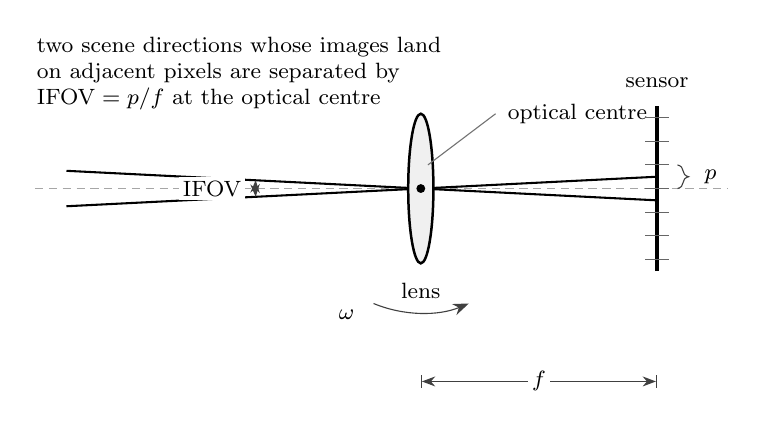
\begin{tikzpicture}[>=Stealth, font=\small, scale=1.0]

% ---- Optical axis ----------------------------------------------------
\draw[black!35, dash pattern=on 3pt off 2pt] (-4.9,0) -- (3.9,0);

% ---- Two object rays, landing on two adjacent pixel centres ----------
% symmetric about the axis: they cross at the optical centre and land at
% y = -0.15 and y = +0.15, which are 0.30 = p apart.
\draw[line width=0.75pt] (-4.5,0.225) -- (0,0) -- (3.0,-0.15);
\draw[line width=0.75pt] (-4.5,-0.225) -- (0,0) -- (3.0,0.15);

% ---- IFOV angle at the optical centre --------------------------------
\draw[{Stealth[length=1.6mm]}-{Stealth[length=1.6mm]}, black!75]
      (-2.0974,0.1048) arc[start angle=177.138, end angle=182.862, radius=2.1];
\node[font=\footnotesize, anchor=east, fill=white, inner sep=1.5pt] at (-2.22,0) {IFOV};

% ---- Lens ------------------------------------------------------------
\draw[line width=0.9pt, fill=black!6] (0,0) ellipse (0.16 and 0.95);
\fill (0,0) circle (1.6pt);
\node[font=\footnotesize, anchor=north] at (0,-1.08) {lens};
\draw[black!55, line width=0.4pt] (0.09,0.30) -- (0.95,0.95);
\node[font=\footnotesize, anchor=west] at (0.98,0.95) {optical centre};

% ---- Sensor ----------------------------------------------------------
\draw[line width=1.2pt] (3.0,-1.05) -- (3.0,1.05);
\foreach \y in {-0.9,-0.6,-0.3,0,0.3,0.6,0.9}{\draw[black!60] (2.85,\y) -- (3.15,\y);}
\node[font=\footnotesize, anchor=south] at (3.0,1.16) {sensor};

% pixel pitch brace between the two boundaries that enclose one pixel
\draw[decorate, decoration={brace, amplitude=4pt, mirror}, black!75]
      (3.26,0.0) -- (3.26,0.30);
\node[font=\footnotesize, anchor=west] at (3.48,0.15) {$p$};

% ---- focal length ----------------------------------------------------
\draw[|<->|, black!75] (0,-2.45) -- (3.0,-2.45);
\node[font=\footnotesize, fill=white, inner sep=1.5pt] at (1.5,-2.45) {$f$};

% ---- rotation --------------------------------------------------------
\draw[-{Stealth[length=2mm]}, black!75]
      (-0.60,-1.46) arc[start angle=247.5, end angle=292.5, radius=1.58];
\node[font=\footnotesize, anchor=east] at (-0.72,-1.60) {$\omega$};

% ---- annotation ------------------------------------------------------
\node[align=left, font=\footnotesize, anchor=north west] at (-5.0,2.05)
  {two scene directions whose images land\\
   on adjacent pixels are separated by\\
   $\mathrm{IFOV} = p/f$ at the optical centre};

\end{tikzpicture}
\caption[Instantaneous field of view and the origin of the motion-blur limit]{Instantaneous field of view. Two scene directions whose images land on adjacent pixels are separated at the optical centre by $\mathrm{IFOV} = p/f$. Rotating the camera at $\omega$ therefore sweeps the image across one pixel in a time $\mathrm{IFOV}/\omega$, which is the exposure ceiling of Equation \ref{eq:tmax}. Drawn with $f = 3$ units and $p = 0.3$ units, so $\mathrm{IFOV} = 5.7^\circ$ as shown; the real values are three orders of magnitude smaller.}
\label{fig:ifov}
\end{figure}

\subsection{Result}

Evaluating Equation \ref{eq:tmax} for the two rotation rates of the rolling-shutter deliverable, 1\textdegree/s from the current 15~fps software configuration and 2.76\textdegree/s from the IMX477 datasheet's 12-bit full-resolution readout limit, gives the second and third columns of Table \ref{tab:light-budget}. The ordering is the reverse of the resolution ordering: the Hawk-eye, which resolves the tether best, tolerates the shortest exposure, because a finer pixel is crossed sooner.

\section{The absolute light requirement}
\label{sec:light-budget}

\subsection{What the datasheet provides}

The Sony IMX477 datasheet specifies sensitivity under a defined test condition, which makes an absolute calculation possible rather than only a relative comparison. Under standard imaging condition I, the sensor images a pattern box of luminance $L_{\mathrm{ref}} = 706$~cd/m\textsuperscript{2} at a colour temperature of 3200~K, through a CM500S infrared-cut filter at $N_{\mathrm{ref}} = \mathrm{F}2.8$, and the sensitivity normalised to a storage time of $t_{\mathrm{ref}} = 1/120$~s is $S = 250$~LSB. The saturation signal is $V_{sat} = 1023$~LSB including an optical-black level of $V_{OB} = 64$~LSB \cite{sony_imx477_datasheet}.

\subsection{Derivation}

The signal is proportional to the exposure, so the luminance-time product that fills the usable range at the reference aperture is

\begin{equation}
(L t)_{sat}(N_{\mathrm{ref}}) = \frac{V_{sat}-V_{OB}}{S} \cdot L_{\mathrm{ref}} \cdot t_{\mathrm{ref}}
= \frac{1023-64}{250} \times 706 \times \frac{1}{120} = 22.57~\mathrm{cd\,s/m^2} .
\label{eq:ltsat-ref}
\end{equation}

Changing the aperture changes the illuminance at the image plane. For an object of luminance $L$ imaged on axis through a lens of f-number $N$ and transmittance $T$,

\begin{equation}
E_{\mathrm{image}} = \frac{\pi\,L\,T}{4\,N^{2}} ,
\label{eq:image-illuminance}
\end{equation}

so at fixed sensor response the saturating luminance-time product scales as $N^{2}$:

\begin{equation}
(L t)_{sat}(N) = (L t)_{sat}(N_{\mathrm{ref}}) \left(\frac{N}{N_{\mathrm{ref}}}\right)^{2} .
\label{eq:ltsat-n}
\end{equation}

For the fitted 8~mm lens wide open, $(L t)_{sat}(1.6) = 22.57 \times (1.6/2.8)^2 = 7.37$~cd\,s/m\textsuperscript{2}; for the 6~mm F1.2, $(L t)_{sat}(1.2) = 4.15$~cd\,s/m\textsuperscript{2}.

The last step converts a luminance the sensor sees into an illuminance a light meter reads, using the Lambertian relation of Equation \ref{eq:lambertian}. For a white card of reflectance $\rho = 0.9$,

\begin{equation}
\boxed{\;H_{sat}(N) = E_v\,t \big|_{sat} = \frac{\pi\,(L t)_{sat}(N)}{\rho}\;}
\label{eq:hsat}
\end{equation}

and the illuminance that reaches full scale within the exposure ceiling is

\begin{equation}
E_{\min} = \frac{H_{sat}}{t_{\max}} .
\label{eq:emin}
\end{equation}

For the fitted configuration this is $H_{sat} = \pi \times 7.37 / 0.9 = 25.72$~lx\,s, and at its 1\textdegree/s ceiling of 11.1~ms, $E_{\min} = 2317$~lx. The same arithmetic with the 6~mm F1.2 gives 14.47~lx\,s and 978~lx. As a scale check, the orbital Sun of Equation \ref{eq:sun-lux} delivers the fitted configuration's $H_{sat}$ in 0.19~ms, nearly two orders of magnitude faster than the 11.1~ms ceiling, which is consistent with full sunlight being far more light than this experiment needs.

\subsection{Assumptions and their effect}

Four assumptions enter Equations \ref{eq:ltsat-ref} to \ref{eq:hsat}, and all of them are conservative in the sense of understating the light needed, except where noted:

\begin{enumerate}
    \item \textbf{Colour temperature.} The datasheet condition uses a 3200~K source, while the specification calls for 5600--6000~K. The sensor's response to the two spectra differs, so the result is an approximation rather than an exact figure.
    \item \textbf{Gain scale.} The datasheet notes that the characteristics are given without the base gain setting applied, and that base gain is defined as the setting at which saturation matches 1023~LSB with an optical-black level of 64~LSB \cite{sony_imx477_datasheet}. Equation \ref{eq:ltsat-ref} treats $S$ and $V_{sat}-V_{OB}$ as being on the same scale.
    \item \textbf{Lens transmittance and vignetting.} Equation \ref{eq:image-illuminance} is the on-axis, $T = 1$ form. Real transmittance below unity and off-axis $\cos^4$ falloff both mean more light is needed than calculated.
    \item \textbf{Target reflectance.} The result is for a white card filling many pixels. The tether is thinner than one pixel on two of the three configurations (Table \ref{tab:sampling}), so its light is diluted with the dark background within the pixel, and it may be considerably darker than $\rho = 0.9$. Both effects increase the requirement.
\end{enumerate}

Because of items 3 and 4 in particular, $E_{\min}$ is a floor, not a target. The on-site test of Section \ref{sec:protocol} measures the real value against the real tether.

\subsection{The other two cameras}

The same calculation cannot be closed from the datasheets of the other two sensors. The Sony IMX296 flyer gives sensitivity as 1146~mV at F5.6 with 1/30~s accumulation and a minimum saturation signal of 1001~mV, but does not state the luminance of the test condition \cite{sony_imx296lqr_flyer}, so the equivalent of Equation \ref{eq:ltsat-ref} cannot be evaluated. Arducam does not identify the Hawk-eye's sensor die at all \cite{arducam_hawkeye_wiki}.

For those two, $H_{sat}$ is carried over from the IMX477 and rescaled for aperture through Equation \ref{eq:ltsat-n}. This assumes the saturation exposure in lx\,s is comparable across the three sensors, which is defensible to first order, because full-well capacity and collected flux both scale with pixel area, so their ratio, the saturation exposure, is roughly area-independent. It is still an assumption about devices of different generations and process technology, it is not backed by any datasheet, and Table \ref{tab:light-budget} labels the affected rows accordingly. Note that the two IMX477 rows carry no such assumption even though they differ in lens, because the aperture scaling of Equation \ref{eq:ltsat-n} is physics applied to the same datasheet constants.

\begin{table}[!ht]
\centering
\small
\caption[Exposure ceiling and light requirement per configuration]{Exposure ceiling from Equation \ref{eq:tmax} with $b_{\max} = 1$~px, and the illuminance that saturates a white card within it from Equation \ref{eq:emin}. The IMX477 rows are anchored in a datasheet; the IMX296 and Hawk-eye rows rescale the IMX477's $H_{sat}$ by aperture. Adjustable lenses are wide open. Computed by \texttt{illumination\_numbers.py}.}
\label{tab:light-budget}
\footnotesize
\setlength{\tabcolsep}{4pt}
\begin{tabular}{lcccccc}
\toprule
\multirow{2}{*}{\textbf{Configuration}} & \multirow{2}{*}{\textbf{$H_{sat}$ [lx\,s]}} & \multicolumn{2}{c}{\textbf{$t_{\max}$ [ms]}} & \multicolumn{2}{c}{\textbf{$E_{\min}$ [lx]}} & \multirow{2}{*}{\textbf{Basis}} \\
\cmidrule(lr){3-4}\cmidrule(lr){5-6}
 & & 1\textdegree/s & 2.76\textdegree/s & 1\textdegree/s & 2.76\textdegree/s & \\
\midrule
\textbf{IMX477 + 8 mm F1.6 (fitted)} & \textbf{25.72} & \textbf{11.1} & \textbf{4.0} & \textbf{2317} & \textbf{6396} & datasheet \cite{sony_imx477_datasheet} \\
IMX477 + 6 mm F1.2     & 14.47 & 14.8 & 5.4  & 978  & 2698 & datasheet \cite{sony_imx477_datasheet} \\
IMX296 + 16 mm F1.4    & 19.69 & 12.4 & 4.5  & 1594 & 4400 & rescaled, assumption \\
IMX296 + 8 mm F1.6     & 25.72 & 24.7 & 9.0  & 1041 & 2873 & rescaled, assumption \\
IMX296 + 6 mm F1.2     & 14.47 & 32.9 & 11.9 & 439  & 1212 & rescaled, assumption \\
Hawk-eye + 5.1 mm F1.8 & 32.55 & 9.0  & 3.3  & 3622 & 9998 & rescaled, assumption \\
\bottomrule
\end{tabular}
\end{table}

\begin{figure}[!ht]
\centering
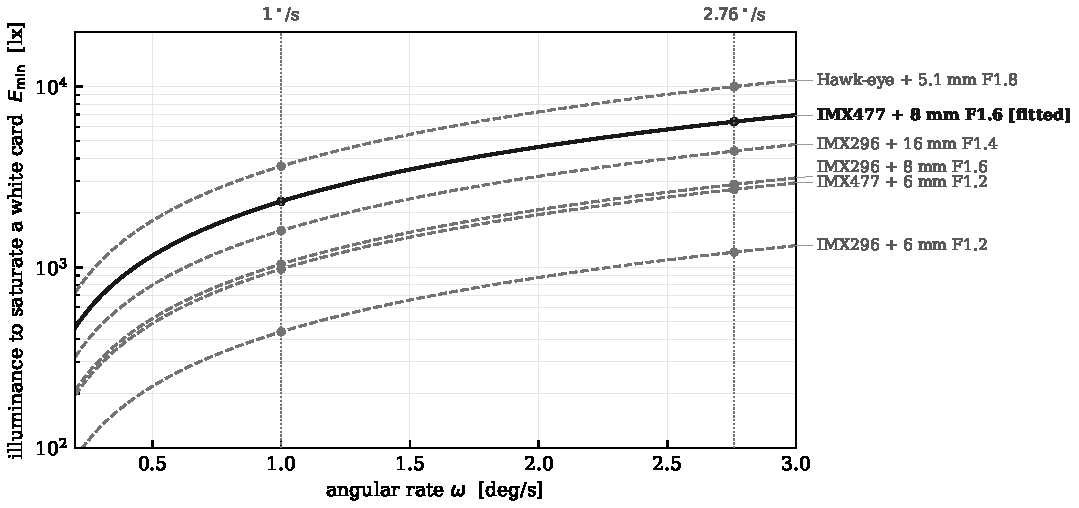
\includegraphics[width=\textwidth]{Images/fig_camera_requirement.pdf}
\caption[Illuminance required as a function of angular rate]{Illuminance required to saturate a white card within the motion-blur ceiling, as a function of angular rate, from Equations \ref{eq:tmax} and \ref{eq:emin}. The requirement is inversely proportional to the available exposure and therefore proportional to $\omega$. Markers show the two rates of Table \ref{tab:light-budget}. Generated by \texttt{make\_figures.py}.}
\label{fig:requirement}
\end{figure}

\subsection{Which configuration sizes the lamp}

The six configurations span 439 to 3622~lx, a range of 3.0 stops, so the lens choice matters as much as the sensor choice. Three readings follow from Table \ref{tab:light-budget}.

\textbf{The Hawk-eye still sets the ceiling}, at 3622~lx, 1.56 times the fitted IMX477 configuration. Its pixel is the smallest of the three sensors, which tightens the exposure ceiling to 9.0~ms, and its fixed F1.8 optic admits $(1.8/1.6)^2 = 1.27$ times less light than the fitted 8~mm lens wide open. If all three cameras are to be exercised in one session, the lamp must be sized for it: roughly \textbf{3600~lx at 1\textdegree/s} and \textbf{10\,000~lx at 2.76\textdegree/s}, measured at the tether position. This is the figure carried into requirement R5 of Chapter \ref{chap:spec}.

\textbf{Dropping the Hawk-eye would lower the requirement to 2317~lx}, the fitted IMX477 configuration, which is 0.6 stops less light.

\textbf{The 8~mm lens costs 1.2 stops relative to the 6~mm} on the same IMX477 sensor, 2317~lx against 978~lx. Both terms push the same way: the longer focal length narrows the IFOV and so shortens the exposure ceiling from 14.8 to 11.1~ms, and F1.6 admits $(1.6/1.2)^2 = 1.78$ times less light than F1.2. What the 8~mm buys in return is sampling, 1.47 pixels across the tether against 1.11 (Table \ref{tab:sampling}), which for a target this close to the sub-pixel limit is the more valuable of the two.

Even the highest requirement, 10\,000~lx, is 3.7 stops below the orbital Sun. The experiment does not need a solar-constant light source; it needs a well-controlled one.

\section{Flicker}
\label{sec:flicker}

\subsection{Mechanism}

A lamp supplied from the alternating-current grid does not emit steadily. Its luminous output rises and falls twice per electrical cycle, so for a supply frequency $f$ the output is periodic with

\begin{equation}
T_{\mathrm{flicker}} = \frac{1}{2f} ,
\label{eq:flicker-period}
\end{equation}

that is 10~ms on a 50~Hz supply and 8.3~ms on a 60~Hz supply \cite{sheinin2018rollingac}. Those periods are the same order of magnitude as every exposure ceiling in Table \ref{tab:light-budget}, which is precisely the regime in which flicker becomes visible in the image.

A rolling-shutter sensor exposes its rows sequentially rather than simultaneously \cite{raspberrypi_camera_docs}. Row $k$ therefore integrates the lamp waveform over a window displaced by $k$ row periods, and when the exposure is short this inter-row delay turns a temporal fluctuation into a spatial pattern across the frame \cite{sheinin2018rollingac}. The same banding mechanism is reported for sources dimmed by pulse-width modulation \cite{zhu2025rifle}. Figure \ref{fig:flicker} computes the result for the IMX477 at the 2.76\textdegree/s exposure ceiling.

\begin{figure}[!ht]
\centering
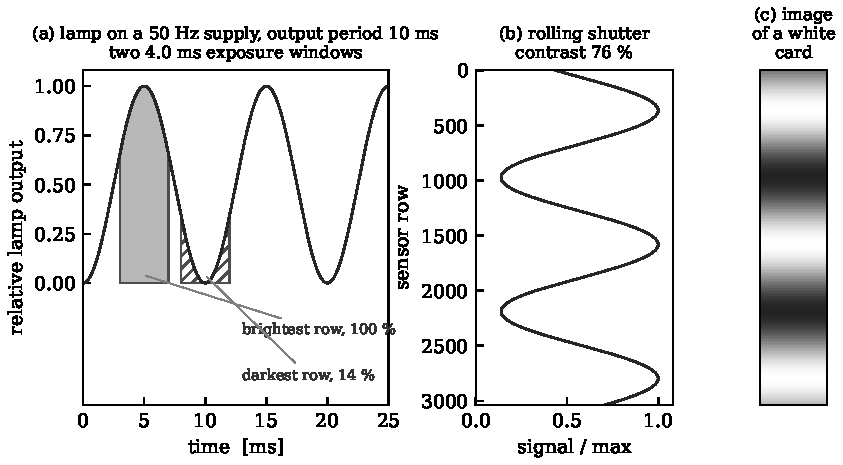
\includegraphics[width=\textwidth]{Images/fig_flicker_banding.pdf}
\caption[Banding produced by an AC-powered lamp on a rolling-shutter sensor]{Flicker banding, computed for a lamp output $L(t) = \sin^{2}(2\pi f t)$ on a 50~Hz supply, an exposure of 4.0~ms, which is the fitted configuration's ceiling at 2.76\textdegree/s, and a 25~ms full-frame readout over 3040 rows, giving a row period of 8.22~\textmu s. (a) The waveform, with the brightest and the darkest 4.0~ms window marked. (b) The signal accumulated by each row. (c) The resulting image of a uniformly lit white card. The 25~ms readout spans 2.5 flicker periods, so 2.5 bands appear. Generated by \texttt{make\_figures.py}.}
\label{fig:flicker}
\end{figure}

\subsection{How bad it gets, and the one exposure that escapes}

Applying the non-uniformity definition of Equation \ref{eq:nu} to the row signals of Figure \ref{fig:flicker}(b) gives a banding contrast that depends strongly on exposure time, as shown in Table \ref{tab:flicker-contrast}. The pattern has a clear structure: when the exposure equals an exact multiple of the flicker period, every row integrates exactly the same amount of light and the banding vanishes, which is the condition Sheinin et al. describe as emulating direct-current illumination \cite{sheinin2018rollingac}. On a 50~Hz supply the computed contrast is exactly zero at 10.0 and 20.0~ms, and rises steeply as the exposure falls below one period: the fitted configuration's 4.0~ms ceiling at 2.76\textdegree/s gives 75.7\%, meaning the darkest band carries about one seventh the signal of the brightest.

\begin{table}[!ht]
\centering
\small
\caption[Banding contrast as a function of exposure time]{Banding contrast across the frame for a 50~Hz supply and a 25~ms readout, from the model of Figure \ref{fig:flicker}. The exposures listed are the ceilings of Table \ref{tab:light-budget} plus the two flicker-free exposures. Computed by \texttt{make\_figures.py}.}
\label{tab:flicker-contrast}
\begin{tabular}{llc}
\toprule
\textbf{Exposure} & \textbf{Where it comes from} & \textbf{Banding contrast} \\
\midrule
3.3 ms  & Hawk-eye ceiling at 2.76\textdegree/s            & 83.0\% \\
\textbf{4.0 ms}  & \textbf{fitted IMX477 ceiling at 2.76\textdegree/s} & \textbf{75.7\%} \\
4.5 ms  & IMX296 + 16 mm ceiling at 2.76\textdegree/s      & 68.5\% \\
5.4 ms  & IMX477 + 6 mm ceiling at 2.76\textdegree/s       & 58.5\% \\
9.0 ms  & Hawk-eye at 1\textdegree/s; IMX296 + 8 mm at 2.76\textdegree/s & 10.9\% \\
10.0 ms & \emph{exactly one flicker period}                & \emph{0.0\%} \\
\textbf{11.1 ms} & \textbf{fitted IMX477 ceiling at 1\textdegree/s}   & \textbf{9.7\%} \\
12.4 ms & IMX296 + 16 mm ceiling at 1\textdegree/s         & 17.6\% \\
14.8 ms & IMX477 + 6 mm ceiling at 1\textdegree/s          & 21.5\% \\
20.0 ms & \emph{exactly two flicker periods}               & \emph{0.0\%} \\
24.7 ms & IMX296 + 8 mm ceiling at 1\textdegree/s          & 12.8\% \\
32.9 ms & IMX296 + 6 mm ceiling at 1\textdegree/s          & 7.6\% \\
\bottomrule
\end{tabular}
\end{table}

Relying on that coincidence is not a viable strategy here, because the exposure time is not free: it is set by Equation \ref{eq:tmax} from the rotation rate under test. The conclusion is that the fixture itself must not flicker.

\subsection{What that requires of the fixture}

For HMI lamps the ballast decides the outcome, and the manufacturer documentation is explicit. ARRI's electronic ballast for the 12/18~kW lamp class, the same class used as the sun simulator at EPOS, lists ``flicker free light'' with a ``typical light ripple max. 3\%'' among its advantages over magnetic ballasts, and offers three modes \cite{arri_eb1218_manual}:

\begin{itemize}
    \item \textbf{50/60 Hz, low noise.} Quieter, but the manual states the light is ``NOT flicker free any more'', with the same camera restrictions as a magnetic ballast.
    \item \textbf{75 Hz, flicker free.} The lamp runs on a 75~Hz square wave and gives constant light, designed for standard film speeds.
    \item \textbf{High speed.} The lamp runs at about 1000~Hz square wave, period 1.00~ms, also flicker free.
\end{itemize}

Given exposures as short as 3.3~ms, the high-speed mode is the appropriate choice, since its 1.00~ms period is short compared with every ceiling in Table \ref{tab:light-budget}. The 75~Hz mode, whose 13.33~ms period exceeds most of those ceilings, is not. For LED fixtures no equivalent statement was found in any reviewed source: the dimming method and pulse-width-modulation frequency must be requested from the manufacturer, and the fixture accepted only after the on-site test.

The global-shutter IMX296 exposes every pixel at once \cite{raspberrypi_camera_docs} and therefore shows no banding, but it is not immune. Its frame brightness still depends on where the exposure window falls within the flicker cycle, as Figure \ref{fig:flicker}(a) shows directly: two windows of equal duration collect 100\% and 14\% of the maximum. On a global-shutter sensor that becomes frame-to-frame brightness variation instead of within-frame banding, which is equally destructive for a stereo pair that must be radiometrically consistent.

\chapter{Specification and Measurement Protocol}
\label{chap:spec}

This chapter states the requirement as eight numbered items, each with the value, the source it comes from, and an acceptance test that can be performed on site with a light meter, a ruler and the project's own cameras. Items whose value is fixed by physics are distinguished from items whose value is a project threshold that may be revised if the available equipment cannot meet it.

\section{Summary of requirements}

\begin{table}[!ht]
\centering
\small
\caption[Summary of the eight illumination requirements]{The eight requirements. ``Physics'' marks a value fixed by the Sun itself; ``project'' marks a threshold adopted for LINKU and open to revision.}
\label{tab:spec}
\begin{tabularx}{\textwidth}{c p{0.21\textwidth} p{0.26\textwidth} X}
\toprule
\textbf{\#} & \textbf{Requirement} & \textbf{Value} & \textbf{Basis} \\
\midrule
R1 & One light direction, no fill & 1 direction, no bounce, no ambient & Physics; Sec. \ref{sec:r1} \\
R2 & Daylight colour & 5600--6000 K nominal, CRI $\geq$ 90, TLCI reported & Project, from Table \ref{tab:vision-labs}; Sec. \ref{sec:r2} \\
R3 & Parallel beam & penumbra $\leq$ 35 mm at 1 m, i.e. $\alpha \leq 2$\textdegree & Project; physics reference 9.3 mm; Sec. \ref{sec:r3} \\
R4 & Uniformity & $NU \leq 5\%$, i.e. $\leq$ 0.14 EV spread & Project, IEC class B; Sec. \ref{sec:r4} \\
R5 & Illuminance at the tether & $\geq$ 3600 lx at 1\textdegree/s; $\geq$ 10\,000 lx at 2.76\textdegree/s & Datasheet derivation, Ch. \ref{chap:cameras}; Sec. \ref{sec:r5} \\
R6 & Stability and flicker & $\leq$ 2\% over the session; flicker-free fixture & Project, IEC class B STI; Sec. \ref{sec:r6} \\
R7 & Black environment & black velvet or molton; lamp out of frame & Project, from Table \ref{tab:vision-labs}; Sec. \ref{sec:r7} \\
R8 & Recorded data & the sheet of Table \ref{tab:record} & Feeds the Blender replica; Sec. \ref{sec:r8} \\
\bottomrule
\end{tabularx}
\end{table}

\section{The requirements in detail}

\subsection{R1: one light direction, hard light, no fill}
\label{sec:r1}

\textbf{Value.} A single key light, or several fixtures aimed strictly parallel as described in Section \ref{sec:multi-lamp}. No fill light, no bounce boards, no practical sources, no residual ambient light.

\textbf{Basis.} In orbit the tether is lit from one direction by one source at effectively infinite distance, and there is no atmosphere to scatter light into the shadows. Earth albedo, the second source that real spacecraft see, is out of scope for this experiment.

\textbf{Acceptance test.} With the lamp off and the room closed, the cameras at the longest exposure to be used must record no discernible scene. Any structure visible in that frame is stray light and must be eliminated before proceeding.

\subsection{R2: daylight colour}
\label{sec:r2}

\textbf{Value.} Manufacturer-rated correlated colour temperature between 5600 and 6000~K, colour rendering index $\geq$ 90. The fixture's TLCI is requested as a reported figure, with no threshold attached.

\textbf{Basis.} Every facility in Table \ref{tab:vision-labs} that states a colour temperature falls in 5600--6000~K, and the EPOS sun simulator is specified at 6000~K with a colour rendering index of 90 \cite{dlr2025eposportfolio}. The Sun's nominal effective temperature is 5772~K \cite{prsa2016iau}. TLCI is requested because the colour rendering index was designed for human vision and the EBU developed TLCI specifically because CRI ``was never intended for use in the television industry'' and has limitations that make it inappropriate there \cite{ebu_tech3355}; no TLCI threshold is set because none was found in any reviewed source. Any fixture whose rated colour temperature lies outside the range is excluded, which rules out tungsten halogen at 3200~K without needing a separate argument.

\textbf{Acceptance test.} Manufacturer specification sheet, confirmed on site with a colour meter if one is available.

\subsection{R3: parallel beam}
\label{sec:r3}

\textbf{Value.} Penumbra width $\leq$ 35~mm measured 1~m behind a shadowing edge, corresponding through Equation \ref{eq:penumbra} to a source angular size of 2\textdegree{} or less.

\textbf{Basis.} The real Sun gives 9.3~mm per metre (Table \ref{tab:penumbra}); the ESA Large Space Simulator achieves a 1.9\textdegree{} collimation angle, equivalent to 33.2~mm per metre \cite{esa_lss}. The 2\textdegree{} threshold is set just outside that reference. Section \ref{sec:falloff} gives the second, independent reason for collimation: without it, the inverse-square gradient across the working volume makes R4 unreachable at any throw a dark room can provide.

\textbf{Acceptance test.} Hold a straight edge 1~m in front of a white card at the tether position and measure the width of the soft transition at the shadow boundary with a ruler. No optical instrument is required.

\textbf{Fixture types that meet it.} Among the reviewed facilities: an HMI spotlight \cite{benninghoff2017epos}, a metal halide arc lamp \cite{park2021tron}, and an LED fixture with a collimator \cite{pauly2022spacelab}. A Fresnel at full spot or a parabolic reflector at the longest available throw is the expected starting point.

\subsection{R4: uniformity over the working volume}
\label{sec:r4}

\textbf{Value.} $NU = (E_{max}-E_{min})/(E_{max}+E_{min}) \leq 5\%$, equivalently a spread of no more than 0.14~EV between the brightest and darkest point of the volume occupied by the LINKU structure and tether.

\textbf{Basis.} Class B of IEC 60904-9, using that standard's own definition, Equation \ref{eq:nu} \cite{iec60904_9_2020}. For comparison, the ESA Large Space Simulator reports $\pm$4\% in plane \cite{esa_lss}, and the GRALS lamp is described as $\pm$5\% \cite{pauly2022spacelab}.

\textbf{Acceptance test.} Incident light meter readings on a three-dimensional grid covering the full width, height and \emph{depth} of the working volume. The depth axis is the one that fails first, per Table \ref{tab:falloff}, and is the one most often omitted from a uniformity check.

\subsection{R5: illuminance at the tether}
\label{sec:r5}

\textbf{Value.} At least 3600~lx for tests at 1\textdegree/s, and at least 10\,000~lx for tests at 2.76\textdegree/s, measured at the tether position with the beam in its final configuration. More is better, since it buys shorter exposures.

\textbf{Basis.} Table \ref{tab:light-budget}, sized for the Hawk-eye as the most demanding of the three cameras. For scale, 10\,000~lx is 3.7 stops below the orbital Sun of Equation \ref{eq:sun-lux}, and the 12~kW HMI at EPOS brackets one solar constant between 7 and 10~m \cite{dlr2025eposportfolio}. This requirement is a floor derived for a white card; the four assumptions of Section \ref{sec:light-budget} all push the real figure upward, which is why the on-site test of Section \ref{sec:protocol} measures it against the real tether.

\textbf{Acceptance test.} Incident light meter at the tether position, plus the camera test of Section \ref{sec:protocol}.

\subsection{R6: stability and freedom from flicker}
\label{sec:r6}

\textbf{Value.} Illuminance stable within 2\% over a capture session after warm-up. The fixture must be flicker-free: for HMI, an electronic ballast in a flicker-free mode, preferably the high-speed mode; for LED, the dimming method and pulse-width-modulation frequency must be declared by the manufacturer and verified on site. Magnetic ballasts, and the 50/60~Hz low-noise mode of an electronic ballast, are excluded \cite{arri_eb1218_manual}.

\textbf{Basis.} The 2\% figure is the class B short-term instability threshold of IEC 60904-9 \cite{iec60904_9_2020}. The flicker requirement follows from Section \ref{sec:flicker}: on a 50~Hz supply the output period of 10~ms is comparable to every exposure ceiling in Table \ref{tab:light-budget}, producing banding contrasts of up to 83\% on a rolling-shutter sensor (Table \ref{tab:flicker-contrast}) and frame-to-frame brightness variation on a global-shutter one.

\textbf{Acceptance test.} Light meter readings at one-minute intervals through a full session, after the warm-up time stated by the manufacturer. Separately, with each camera: photograph a uniformly lit white card at the shortest exposure to be used, and check for horizontal bands on the rolling-shutter cameras and for brightness variation across a burst of frames on the global-shutter camera.

\subsection{R7: black, non-reflective environment}
\label{sec:r7}

\textbf{Value.} Black velvet or molton behind and around the structure and on all supports inside the camera field. No light spill onto walls, floor or ceiling. The fixture itself outside the camera field of view.

\textbf{Basis.} Black molton curtain, carpet and robot wrapping are what DLR EPOS uses \cite{benninghoff2017epos,dlr2025eposportfolio}, black commando curtains are what Stanford TRON uses \cite{park2021tron}, and black velvet scored best among the background materials the SnT Zero-G Lab tested with the Raspberry Pi HQ camera \cite{pauly2022spacelab}. TRON also reports the sun lamp casting a flare across the image when the camera points near it \cite{park2021tron}, which is the reason for keeping the fixture out of frame. IEC 60904-9 independently lists reflections from dark-room walls among the factors that invalidate a measured classification \cite{iec60904_9_2020}.

\textbf{Acceptance test.} Covered by the R1 stray-light test, plus visual inspection of each camera's framing for the fixture and for specular returns from supports.

\subsection{R8: recorded data}
\label{sec:r8}

\textbf{Value.} The record sheet of Table \ref{tab:record}, completed during the session.

\textbf{Basis.} These values are the inputs the Blender replica needs in order to reproduce the same light instead of a placeholder, and they are also what makes the experiment reproducible.

\section{Several lamps for a long set}
\label{sec:multi-lamp}

The requirement of R1 is one light \emph{direction}, not one fixture. In orbit the whole tether receives sunlight at the same incidence angle and the same irradiance, because the source is effectively at infinity. When a single beam cannot cover the illuminated length of the tether, several identical fixtures may be placed in a row, all aimed parallel, at equal distance and equal incidence angle. Among the reviewed facilities, INVERITAS is reported to use six motorised spotlights \cite{pauly2022spacelab}, though that entry rests on a secondary source. No reviewed source describes how a parallel row is aligned, so the rules below follow from the geometry of Chapter \ref{chap:sun} rather than from a precedent.

\begin{figure}[!ht]
\centering
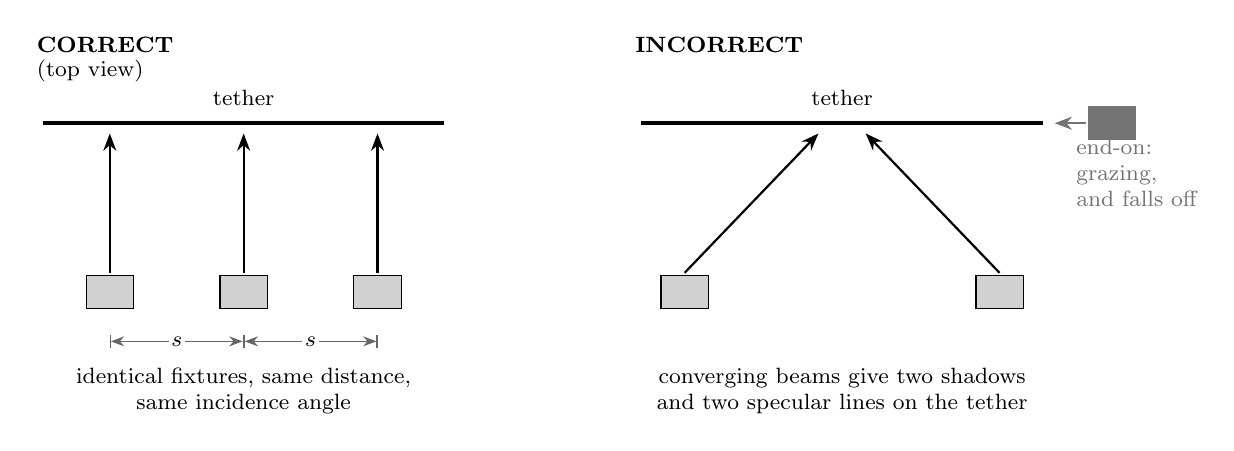
\begin{tikzpicture}[>=Stealth, font=\small, scale=1.0]

% =============== CORRECT ===============
\begin{scope}
\node[font=\footnotesize\bfseries, anchor=west] at (-0.3,2.35) {CORRECT};
\node[font=\footnotesize, anchor=west] at (-0.3,2.02) {(top view)};
\draw[line width=1.6pt] (-0.1,1.35) -- (5.0,1.35);
\node[font=\footnotesize, anchor=south] at (2.45,1.45) {tether};
\foreach \x in {0.75,2.45,4.15}{
  \draw[-{Stealth[length=2.2mm]}, line width=0.8pt] (\x,-0.55) -- (\x,1.22);
  \draw[fill=black!18] (\x-0.3,-1.0) rectangle (\x+0.3,-0.58);
}
\draw[|<->|, black!60] (0.75,-1.42) -- (2.45,-1.42);
\draw[|<->|, black!60] (2.45,-1.42) -- (4.15,-1.42);
\node[font=\footnotesize, fill=white, inner sep=1pt] at (1.6,-1.42) {$s$};
\node[font=\footnotesize, fill=white, inner sep=1pt] at (3.3,-1.42) {$s$};
\node[align=center, font=\footnotesize] at (2.45,-2.05) {identical fixtures, same distance,\\same incidence angle};
\end{scope}

% =============== INCORRECT ===============
\begin{scope}[xshift=7.6cm]
\node[font=\footnotesize\bfseries, anchor=west] at (-0.3,2.35) {INCORRECT};
\draw[line width=1.6pt] (-0.1,1.35) -- (5.0,1.35);
\node[font=\footnotesize, anchor=south] at (2.45,1.45) {tether};
% converging lamps
\draw[-{Stealth[length=2.2mm]}, line width=0.8pt] (0.45,-0.55) -- (2.15,1.22);
\draw[fill=black!18] (0.15,-1.0) rectangle (0.75,-0.58);
\draw[-{Stealth[length=2.2mm]}, line width=0.8pt] (4.45,-0.55) -- (2.75,1.22);
\draw[fill=black!18] (4.15,-1.0) rectangle (4.75,-0.58);
% end-on lamp
\draw[-{Stealth[length=2.2mm]}, line width=0.8pt, black!55] (5.55,1.35) -- (5.15,1.35);
\draw[fill=black!18, black!55] (5.58,1.14) rectangle (6.18,1.56);
\node[font=\footnotesize, anchor=west, black!55, align=left] at (5.3,0.72) {end-on:\\grazing,\\and falls off};
\node[align=center, font=\footnotesize] at (2.45,-2.05) {converging beams give two shadows\\and two specular lines on the tether};
\end{scope}

\end{tikzpicture}
\caption[Correct and incorrect multi-lamp layouts]{Multi-lamp layout, seen from above. Left: fixtures in a row, all aimed parallel at equal spacing $s$ and equal distance, reproduce a single light direction along the whole tether. Right: beams arriving from different angles each produce their own shadow and their own specular highlight on a cylindrical tether, so the thread can appear doubled in the image; and a fixture placed at one end illuminates the tether at grazing incidence with inverse-square falloff along its length.}
\label{fig:multilamp}
\end{figure}

Three configurations are excluded:

\begin{enumerate}
    \item \textbf{Converging beams.} Each light direction produces its own shadow and, on a specular cylindrical tether, its own highlight line. Two highlight lines on a target that is itself about one pixel wide (Table \ref{tab:sampling}) can present as a doubled thread, which is a failure mode the stereo matching stage is not designed to handle.
    \item \textbf{Mixed fixtures or colour temperatures along the row.} This violates R2 locally even if each fixture passes individually, and it makes the colour of the tether a function of position.
    \item \textbf{A fixture at one end, shining along the tether.} The incidence angle becomes grazing and Equation \ref{eq:inverse-square} applies along the tether's own length, so the far end is both dimmer and differently shaded.
\end{enumerate}

The spacing $s$ is determined on site, not in advance: measure the illuminance profile of one fixture along the tether axis, then space the fixtures so that the summed profile, including the overlap regions where contributions add, satisfies R4 over the whole illuminated length. The number of fixtures required is the illuminated length divided by the usable width of one beam, where usable means the portion that keeps the summed profile within R4.

\todo[inline]{Pending: the illuminated tether length in the dark room and the usable beam width of the candidate fixture are both unknown, so the fixture count cannot be stated here. Determine both before the session is scheduled.}

\section{Measurement protocol}
\label{sec:protocol}

The order matters: the geometric requirements are settled before the photometric ones, because moving a fixture to fix uniformity changes the illuminance, while dimming it does not change the uniformity.

\begin{enumerate}
    \item \textbf{Darken.} Close the room, cover all ambient sources, install the black background and wrap the supports. Verify R1 with the stray-light frame.
    \item \textbf{Warm up.} Run the fixture for the manufacturer's stated warm-up time before any measurement. For HMI this is several minutes; EBU recommends at least 30 minutes for the spectroradiometer itself where one is used \cite{ebu_tech3355}.
    \item \textbf{Set the beam.} Position and aim the fixture at the longest throw the room allows, at full spot. Verify R3 with the straight-edge and ruler test at 1~m.
    \item \textbf{Map uniformity.} Measure the illuminance grid over the working volume, including the depth axis, and compute $NU$ from Equation \ref{eq:nu}. If R4 fails, adjust the beam or add fixtures per Section \ref{sec:multi-lamp} and repeat from step 3.
    \item \textbf{Record the level.} With the geometry settled, record the illuminance at the tether position and check it against R5.
    \item \textbf{Check flicker.} With each camera in turn, at base gain and fixed white balance, photograph a uniformly lit white card at the shortest exposure that will be used. Check for horizontal bands on the IMX477 and the Hawk-eye, and for brightness variation over a burst of frames on the IMX296.
    \item \textbf{Check against the real tether.} Install the tether proxy at its working position. With each camera at base gain, fixed white balance and manual exposure set to its ceiling from Table \ref{tab:light-budget}, confirm that the tether is resolved without saturating and without visible blur. This step replaces the white-card estimate of Section \ref{sec:light-budget} with a measured value, and it is the one that validates or corrects the two assumption-based rows of that table.
    \item \textbf{Monitor stability.} Log illuminance at one-minute intervals for the duration of a representative session and verify R6.
    \item \textbf{Complete the record sheet} of Table \ref{tab:record}.
\end{enumerate}

\section{Record sheet}
\label{sec:record}

\begin{table}[!ht]
\centering
\small
\caption[Data to record during the dark-room session]{Record sheet. The last column indicates which requirement or downstream consumer each entry serves.}
\label{tab:record}
\begin{tabularx}{\textwidth}{X l p{0.14\textwidth} p{0.14\textwidth}}
\toprule
\textbf{Quantity} & \textbf{Unit} & \textbf{Value} & \textbf{Serves} \\
\midrule
Fixture make, model, modifier, quantity, ballast or driver mode & text & & R2, R3, R6 \\
Working volume of the structure: width, height, depth & m & & R4 \\
Illuminated tether length & m & & Sec. \ref{sec:multi-lamp} \\
Fixture throw and incidence angle relative to structure and cameras & m, \textdegree & & R3, Blender \\
Illuminance at the tether position & lx & & R5, Blender \\
Uniformity grid: minimum and maximum & lx & & R4 \\
Measured correlated colour temperature & K & & R2, Blender \\
Penumbra width at 1 m & mm & & R3, Blender \\
Illuminance log: minimum and maximum over the session & lx & & R6 \\
Per camera: model, lens, exposure time, analogue gain, white balance & text & & R5, R6 \\
Flicker check result per camera & pass/fail & & R6 \\
\bottomrule
\end{tabularx}
\end{table}

\section{What this hands to the Blender deliverable}
\label{sec:to-blender}

The companion deliverable on Blender simulation validation renders the same scene and compares it against the photographs taken under this specification. Four of the recorded quantities become its laboratory-condition light parameters, replacing the placeholder values it currently carries:

\begin{itemize}
    \item \textbf{Illuminance at the tether}, converted to the irradiance units Blender's Sun lamp expects. For a source of known correlated colour temperature the conversion is a division by that source's luminous efficacy, the quantity defined in Equation \ref{eq:efficacy}; for the orbital-condition render the deliverable continues to use the AM0 value of 1361~W/m\textsuperscript{2} directly.
    \item \textbf{Measured colour temperature}, as the blackbody shader temperature.
    \item \textbf{Fixture position and aim}, as the lamp transform in the scene.
    \item \textbf{Penumbra width at 1 m}, which fixes the angular size of the Blender light, the parameter that controls shadow softness, through Equation \ref{eq:penumbra}.
\end{itemize}

The last of these is worth emphasising, because it is the parameter most often left at its default in a render: a Blender sun with the wrong angular size produces shadows of the wrong sharpness, and the resulting image will not match the photograph no matter how accurate the irradiance value is.

\chapter{Conclusion}

\section{What this document establishes}

The illumination for the LINKU dark-room experiment is now specified as eight numbered, individually testable requirements (Table \ref{tab:spec}), stated in the units a lighting specialist works in and traceable item by item to either a primary source or an explicit project decision. Three results are worth restating.

\textbf{The Sun, expressed as a lighting fixture.} Integrating the ASTM E490 AM0 spectrum against the CIE photopic luminous efficiency function gives a luminous efficacy of 97.59~lm/W for extraterrestrial sunlight, and therefore an illuminance of 132\,800~lx at the IAU nominal solar constant (Equation \ref{eq:sun-lux}). Its angular diameter of 0.533\textdegree{} sets a shadow penumbra of 9.3~mm per metre (Equation \ref{eq:penumbra}). These two numbers are what a lamp has to be compared against, and neither of them appears in the astrophysical literature in a form a lighting professional can use.

\textbf{The experiment does not need solar intensity; it needs solar geometry.} The light level required at the tether is between 439 and 10\,000~lx depending on camera and rotation rate (Table \ref{tab:light-budget}), the highest of which is 3.7 stops below real sunlight. What cannot be relaxed is the geometry: a beam that is not collimated cannot hold 5\% uniformity across the depth of the structure at any throw a dark room can offer (Table \ref{tab:falloff}), and a fixture that flickers produces banding contrasts of up to 83\% at the exposures this experiment is forced to use (Table \ref{tab:flicker-contrast}).

\textbf{The lens matters as much as the sensor, and the Hawk-eye sizes the lamp.} Across the six sensor-and-lens combinations the requirement spans 439 to 3622~lx, a range of 3.0 stops. The Arducam Hawk-eye is the most demanding at 3622~lx, 1.56 times the fitted IMX477 configuration, because its finer pixel tightens the motion-blur ceiling and its fixed F1.8 optic admits less light than the 8~mm wide open. Any session intended to cover all three cameras must be sized for it. On the same IMX477 sensor, the fitted 8~mm F1.6 costs 1.2 stops against the 6~mm F1.2, and buys 1.47 pixels across the tether instead of 1.11.

\section{Confidence in each part}

\begin{table}[!ht]
\centering
\small
\caption[Confidence in the main results]{Where each principal result stands.}
\label{tab:confidence}
\begin{tabularx}{\textwidth}{p{0.32\textwidth} p{0.13\textwidth} X}
\toprule
\textbf{Result} & \textbf{Status} & \textbf{Basis or limitation} \\
\midrule
132\,800 lx, 0.533\textdegree, 9.3 mm/m & Firm & Computed from primary data \cite{astm_e490_data,cie_vlambda,prsa2016iau}. \\
IEC classes and intervals & Firm & Read in the official preview of the standard \cite{iec60904_9_2020}. \\
Uniformity and collimation argument & Firm & Follows from the inverse-square law and the IEC definition. \\
978 lx for the IMX477 & Derived & Anchored in the Sony datasheet \cite{sony_imx477_datasheet}; four stated assumptions, all of which raise the real figure. \\
439 and 3622 lx for the other two & Assumption & No usable datasheet constants exist for either sensor; rescaled from the IMX477 by aperture. \\
Flicker contrasts & Firm model & Computed from an explicit waveform model; validated by the zero-contrast result at exactly one flicker period, which matches the published condition \cite{sheinin2018rollingac}. \\
EPOS, TRON, ESA LSS, ORION, Zero-G rows & Verified & Read in documents by the facilities' own operators. \\
INVERITAS and GRALS rows & Unverified & Secondary source only \cite{pauly2022spacelab}; both originals refused automated download. \\
\bottomrule
\end{tabularx}
\end{table}

\section{Open items}

The specification is complete; four quantities must be measured before it can be closed, and all four are marked in the text where they arise:

\begin{enumerate}
    \item The working-volume depth of the LINKU structure and the maximum fixture throw available in the dark room, which together determine whether R4 is reachable with the candidate fixture (Section \ref{sec:falloff}).
    \item The illuminated tether length and the usable beam width of the chosen fixture, which determine the number of fixtures required (Section \ref{sec:multi-lamp}).
    \item The measured illuminance needed against the real tether rather than a white card, which replaces the floor of Table \ref{tab:light-budget} with a measured value and tests the two assumption-based rows (Section \ref{sec:protocol}, step 7).
    \item The dimming method and pulse-width-modulation frequency of any LED fixture offered, for which no reviewed source gives a safe value (Section \ref{sec:r6}).
\end{enumerate}

Two external dependencies remain outside this document's control and are tracked in the project work plan: the completion of the LINKU structure by a team member, and confirmation of the dark-room date by the teaching staff.

\appendix

\chapter{Symbols and Constants}
\label{app:symbols}

\begin{table}[!ht]
\centering
\small
\caption[Symbols used in this document]{Symbols, in order of first appearance.}
\label{tab:symbols}
\begin{tabularx}{\textwidth}{p{0.10\textwidth} p{0.115\textwidth} X l}
\toprule
\textbf{Symbol} & \textbf{Unit} & \textbf{Meaning} & \textbf{First use} \\
\midrule
$\Phi_v$   & lm            & Luminous flux                                   & Eq. \ref{eq:lumen} \\
$V(\lambda)$ & --          & CIE photopic spectral luminous efficiency       & Eq. \ref{eq:lumen} \\
$K_m$      & lm/W          & Maximum luminous efficacy, 683                  & Eq. \ref{eq:lumen} \\
$K$        & lm/W          & Luminous efficacy of a given spectrum           & Eq. \ref{eq:efficacy} \\
$I_v$      & cd            & Luminous intensity                              & Eq. \ref{eq:candela} \\
$E_v$      & lx            & Illuminance                                     & Eq. \ref{eq:lux} \\
$L_v$      & cd/m\textsuperscript{2} & Luminance                             & Eq. \ref{eq:luminance} \\
$\rho$     & --            & Reflectance of a Lambertian surface             & Eq. \ref{eq:lambertian} \\
$H_v$      & lx\,s         & Photometric exposure, $E_v t$                   & Eq. \ref{eq:exposure} \\
$E_{e,\lambda}$ & W/(m\textsuperscript{2}nm) & Spectral irradiance           & Eq. \ref{eq:lux-from-spectrum} \\
$\alpha$   & \textdegree   & Angular diameter of a source                    & Eq. \ref{eq:angular-diameter} \\
$w$        & mm            & Penumbra width                                  & Eq. \ref{eq:penumbra} \\
$L$        & m             & Distance behind an occluding edge               & Eq. \ref{eq:penumbra} \\
$D$        & m             & Fixture throw; also camera working distance     & Eq. \ref{eq:inverse-square} \\
$\Delta z$ & m             & Depth of the working volume                     & Fig. \ref{fig:falloff} \\
$NU$       & \%            & Spatial non-uniformity of irradiance            & Eq. \ref{eq:nu} \\
$p$        & \textmu m     & Pixel pitch                                     & Eq. \ref{eq:ifov} \\
$f$        & mm            & Lens focal length                               & Eq. \ref{eq:ifov} \\
$W$        & mm            & Active sensor width, $p \cdot N_h$              & Eq. \ref{eq:fov} \\
$N$        & --            & Lens f-number                                   & Eq. \ref{eq:image-illuminance} \\
$\mathrm{GSD}$ & mm        & Ground sample distance                          & Eq. \ref{eq:gsd} \\
$\omega$   & \textdegree/s & Camera angular rate                             & Eq. \ref{eq:blur} \\
$b$        & px            & Motion blur                                     & Eq. \ref{eq:blur} \\
$t_{\max}$ & s             & Exposure ceiling                                & Eq. \ref{eq:tmax} \\
$H_{sat}$  & lx\,s         & Exposure that saturates the sensor              & Eq. \ref{eq:hsat} \\
$E_{\min}$ & lx            & Illuminance required within $t_{\max}$          & Eq. \ref{eq:emin} \\
$T_{\mathrm{flicker}}$ & s & Period of the lamp's luminous output            & Eq. \ref{eq:flicker-period} \\
\bottomrule
\end{tabularx}
\end{table}

\begin{table}[!ht]
\centering
\small
\caption[Constants used in the calculations]{Every constant entering \texttt{illumination\_numbers.py}, with its source.}
\label{tab:constants}
\begin{tabularx}{\textwidth}{p{0.19\textwidth} p{0.20\textwidth} X}
\toprule
\textbf{Constant} & \textbf{Value} & \textbf{Source} \\
\midrule
$K_m$ & 683 lm/W & SI definition of the candela \\
$\mathcal{S}^{\,\mathrm{N}}_{\odot}$ & 1361 W/m\textsuperscript{2} & IAU 2015 Resolution B3 \cite{prsa2016iau} \\
$\mathcal{R}^{\,\mathrm{N}}_{\odot}$ & 695\,700 km & IAU 2015 Resolution B3 \cite{prsa2016iau} \\
$\mathcal{T}^{\,\mathrm{N}}_{\mathrm{eff}\odot}$ & 5772 K & IAU 2015 Resolution B3 \cite{prsa2016iau} \\
au & 149\,597\,870.7 km & IAU 2012 Resolution B2 \\
IMX477 sensitivity $S$ & 250 LSB & Sony datasheet, sec. 10-1 \cite{sony_imx477_datasheet} \\
IMX477 $V_{sat}$ & 1023 LSB & Sony datasheet, sec. 10-1 \cite{sony_imx477_datasheet} \\
IMX477 $V_{OB}$ & 64 LSB & Sony datasheet, sec. 10-1 note 2 \cite{sony_imx477_datasheet} \\
Test luminance $L_{\mathrm{ref}}$ & 706 cd/m\textsuperscript{2}, 3200 K & Sony datasheet, cond. I, sec. 11-3-1 \cite{sony_imx477_datasheet} \\
Test aperture, time & F2.8, 1/120 s & Sony datasheet, sec. 11-3-1 and 11-4-1 \cite{sony_imx477_datasheet} \\
Pixel pitches & 1.55, 3.45, 0.80 \textmu m & \cite{raspberrypi_camera_docs}, \cite{arducam_hawkeye_wiki} \\
Resolutions & 4056, 1456, 9152 px & \cite{raspberrypi_camera_docs}, \cite{arducam_hawkeye_wiki} \\
Lenses & 8.0 mm F1.6 (fitted); 6.0 mm F1.2; 16.0 mm F1.4; 5.1 mm F1.8 & Arducam C1508ZM04 page and LINKU D5 Camera System Report; \cite{raspberrypi_camera_docs}; project optical comparator \\
Working distance & 3.5 m & Blender replica of the enclosure \\
Tether diameter & 1.0 mm & default in \texttt{camera\_dof\_visualizer.py} \\
Angular rates & 1.0 and 2.76 \textdegree/s & rolling-shutter deliverable \\
White card $\rho$ & 0.9 & assumption, stated in Sec. \ref{sec:light-budget} \\
\bottomrule
\end{tabularx}
\end{table}

\FloatBarrier

\chapter{Findings in the Project Code and Documentation}
\label{app:findings}

Three discrepancies were found while assembling the camera parameters of Chapter \ref{chap:cameras}. None originates in this document, and all three are recorded here.

\section*{In the documentation}

\textbf{Field of view quoted for the 8 mm lens.} Chapter 5 of the LINKU D5 Camera System Report \cite{linku_d5_camera_report} states that the Arducam C1508ZM04 gives ``approximately 58.4\textdegree{} in the horizontal direction and 44.6\textdegree{} in the vertical direction'' on the IMX477. Those are the lens manufacturer's figures for the lens's own 2/3'' optical format. The same specification separately gives 44\textdegree(H) for a 1/2.3'' IMX477 \cite{arducam_c1508zm04}, and the geometry of Equation \ref{eq:fov} with the 6.287~mm active width gives 42.9\textdegree(H) $\times$ 32.8\textdegree(V). The quoted horizontal figure therefore overstates the real field of view by about 36\%. Anything derived from it, such as the angular coverage of the tether deployment region, should be rechecked.

\section*{In the optical comparator}

The following are in \texttt{calculate\_cam/camera\_dof\_visualizer.py}.

\begin{enumerate}
    \item \textbf{Hawk-eye sensor label.} The entry is named ``Arducam Hawk-eye (OV64A40)'' with \texttt{pixel\_size\_um: 1.4} annotated as estimated. The OV64A40 is a different product, the 64MP OwlSight, of optical format 1/1.32'' and pixel pitch 1.008~\textmu m. The Hawk-eye's documented pitch is 0.80~\textmu m at optical format 1/1.7'' \cite{arducam_hawkeye_wiki}, which also equals that entry's own \texttt{sensor\_width\_mm} divided by \texttt{resolution\_h}. Because every computation in that file derives pixel pitch from width over resolution rather than reading the \texttt{pixel\_size\_um} field, the computed outputs are correct; only the label and the annotated field are wrong.
    \item \textbf{Minimum object distance of the 6 mm lens.} The entry reads \texttt{"mod\_mm": 0.2} with the comment ``minimum focus distance 0.2 mm''. The manufacturer value is 0.2~\textbf{m}, that is 200~mm \cite{raspberrypi_camera_docs}. The field is used as \texttt{max(near, lens["mod\_mm"]/1000)}, so the stored value of 0.2~mm disables the near-distance clamp that the field exists to apply. This one does affect the tool's output at short distances. It does not affect any number in this document, which works at a 3.5~m working distance, well beyond either value.

    The origin of the error is traceable: the Arducam product page for the HQ camera bundle with this lens, SKU B0240, lists ``MOD 0.2mm'', while Arducam's own page for the same lens sold separately lists ``MOD: 0.2m''. The comparator reproduced the typo rather than introducing it.

    \item \textbf{Stored field of view of the 6 mm lens.} The entry reads \texttt{"fov\_h\_deg": 65.0}, taken from the same Arducam bundle page. Equation \ref{eq:fov} with that page's own stated sensor area gives 55.3\textdegree{} horizontal, and Raspberry Pi publishes 55\textdegree{} for the same focal length on the same camera \cite{raspberrypi_camera_docs}; 65\textdegree{} is close to the 66.4\textdegree{} \emph{diagonal}. Table \ref{tab:fov-check} sets out the comparison. The same mismatch exists for other entries in that file, whose stored \texttt{fov\_h\_deg} values are manufacturer figures for assorted optical formats rather than values derived for the sensor each lens is paired with. The field is used only for the displayed field-of-view read-out and for the depth-of-field plot's horizontal extent; the thread-pixel and 1~px-limit computations derive their geometry from \texttt{sensor\_width\_mm}, \texttt{resolution\_h} and \texttt{focal\_length\_mm}, so those outputs are unaffected.
\end{enumerate}

\FloatBarrier

\chapter{Complete Numeric Output}
\label{app:numeric}

The following is the unedited output of \texttt{illumination\_numbers.py}, followed by the flicker-contrast figures emitted by \texttt{make\_figures.py}. Every table in this document is drawn from it. Both scripts, and the two data files they read, are in \texttt{Sources/data/}.

{\scriptsize\verbatiminput{Sources/data/numeric_output.txt}}


\bibliographystyle{ieeetr}
\bibliography{bibs/sample}

\end{document}
